\chapter{Molecular mechanisms of aspartate limitation}
\label{chap2}
\textit{Aspartate limitation, a level of aspartate insufficient to sustain maximal cell proliferation.}


\section{Introduction}
Cells require aspartate for protein synthesis and as a metabolic substrate to fuel proliferation.
However, unlike most amino acids, aspartate levels are dictated by cellular metabolism and are influenced by many perturbations that alter said metabolism.
Metabolic perturbations leading to a small decrease in aspartate synthesis capacity does not result in full aspartate depletion; rather, it results in a downwards adjustment of the aspartate level as well as cell proliferation.
This aspartate to proliferation correlation has been observed in several cell lines using various ways of constraining aspartate synthesis \cite{Sullivan2015-xf, Birsoy2015-pg, Gui2016-ca}.
Many of these constraints also result in decreased \NAD{}/NADH ratio; however, aspartate levels can be uncoupled from the \NAD{}/NADH ratio to show a causal link between aspartate levels and cell proliferation \cite{Sullivan2018-gz, Garcia-Bermudez2018-mj}.

Interestingly, aspartate levels are not only related to cell proliferation but has also been associated with modifications to cell function in multiple biological processes, including stem cells \cite{Tournaire2022-ut, Arnold2022-ft}, immune cells \cite{Bailis2019-mf}, endothelial cells \cite{Diebold2019-hh}, and cancer \cite{Helenius2021-ht}.
The sum of these observations provide impetus for studying the underlying reasons for the ability of aspartate levels to ``control'' proliferation rate.
Aspartate's role as a substrate for asparagine and nucleotide synthesis is known, its requirement for protein synthesis is self-evident and simultaneously it is cycled between the cytoplasm and the mitochondrial matrix to transfer electrons into the matrix via. the malate-aspartate shuttle.
It is unknown if these roles of aspartate are involved in its coupling to proliferation, but this knowledge would be useful to establish the mechanism of aspartate limitation.

In this chapter the concept of aspartate limitation is investigated.
A stable correlation between intracellular aspartate levels and proliferation is established, the flux towards the different fates of aspartate is estimated, a mix of salvageable fates of aspartate is characterized and their individual influence on rescuing aspartate limitation is determined.
Finally, aspartate limitation's effect on tRNA aminoacylation levels is measured and its effect on integrated stress response is surveyed.




\section{Results}
\subsection{Mitochondrial inhibition induces a titratable aspartate limitation}
Aspartate limitation was induced with complex I inhibitor rotenone in two experiments measuring intracellular aspartate and the \NAD{}/NADH ratio alongside cell counts to calculate the proliferation rate between time zero and 2, 3, 4 and 5 days (figure \ref{fig:ch2:NAD_Asp_time}).
Proliferation rate adjusts in accordance with the rotenone dose and can be partially rescued with pyruvate.
For the highest dose of rotenone, proliferation decreases over time, reflecting the time it takes before steady-state proliferation is reached.

Intracellular aspartate decreases to correlate with proliferation rate (figure \ref{fig:ch2:Asp_by_day}) but then recovers slightly over time, likely due to media conditioning and rotenone breakdown (appendix figure \ref{fig:ch2:app:Rot_by_day}).
Intracellular asparagine appear to be affected similarly to aspartate (appendix figure \ref{fig:ch2:app:Metab_by_day}).
Throughout the experiment intracellular aspartate and \NAD{}/NADH ratio correlate as expected (figure \ref{fig:ch2:NAD_Asp_corr}).

\begin{figure}
    \centering
    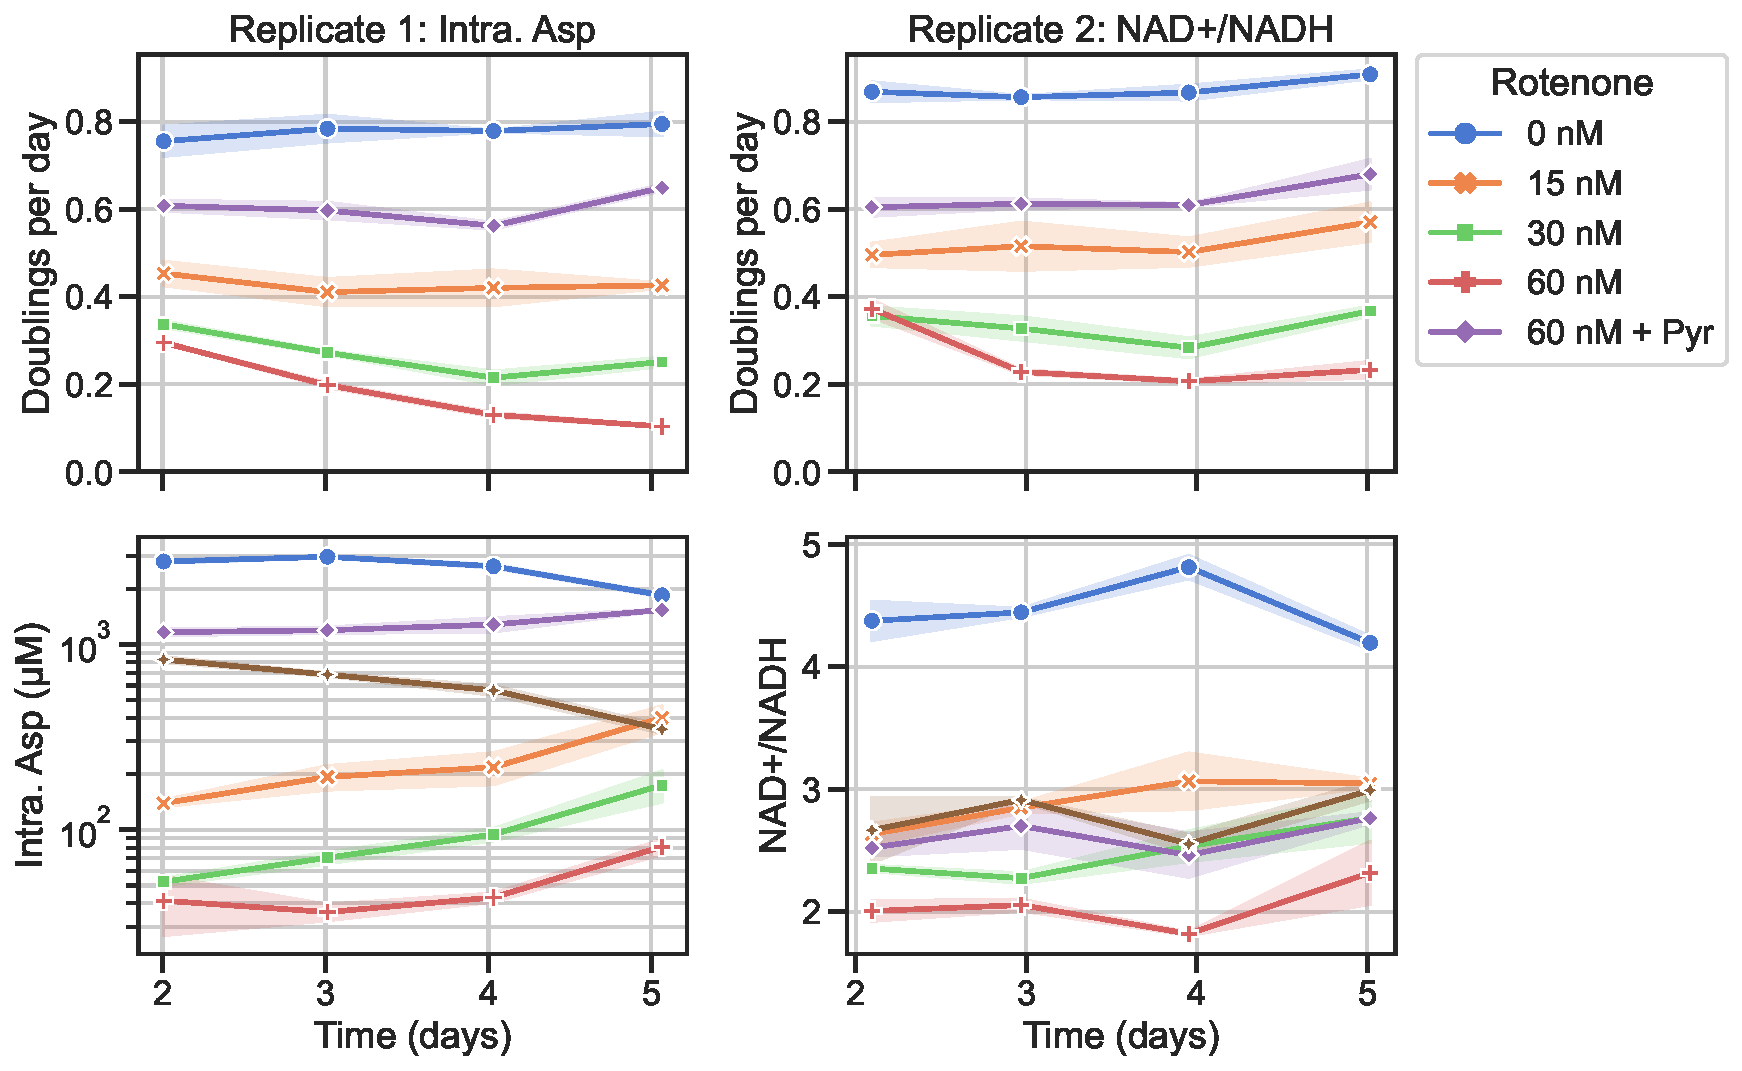
\includegraphics[width=0.8\textwidth]{figures/chap2/prlfr-asp-NAD-NADH-time_rep1-2.pdf}
    \caption[Aspartate, \NAD{}/NADH ratio over time after rotenone.]{
    Rotenone induces aspartate limitation in H1299 cells.
    In replicate one (left column), proliferation rate and intracellular aspartate concentration were determined over time.
    In replicate two (right column), proliferation rate and the \NAD{}/NADH ratio were determined over time.
    For rescue, 2 mM pyruvate was used.
    }
    \label{fig:ch2:NAD_Asp_time}
\end{figure}

\begin{figure}
    \centering
    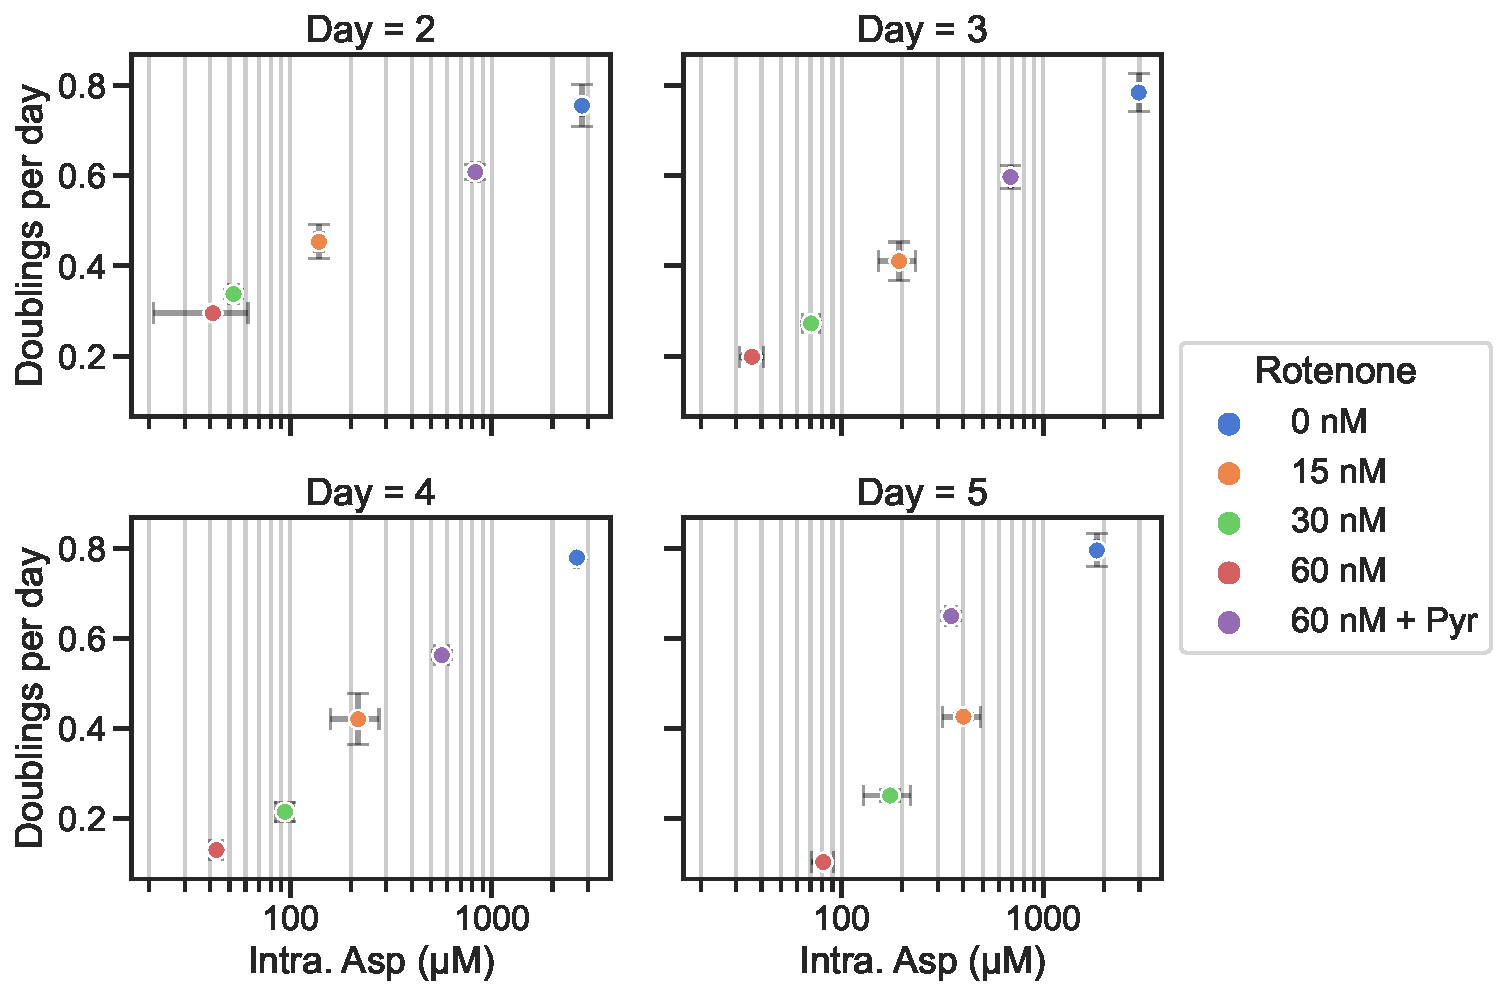
\includegraphics[width=0.72\textwidth]{figures/chap2/intra-asp-prlfr_rep1-byday.pdf}
    \caption[Aspartate levels correlates with proliferation rate.]{
    Correlation between the intracellular aspartate concentration and proliferation rate for data in figure \ref{fig:ch2:NAD_Asp_time}.
    }
    \label{fig:ch2:Asp_by_day}
\end{figure}

\begin{figure}
    \centering
    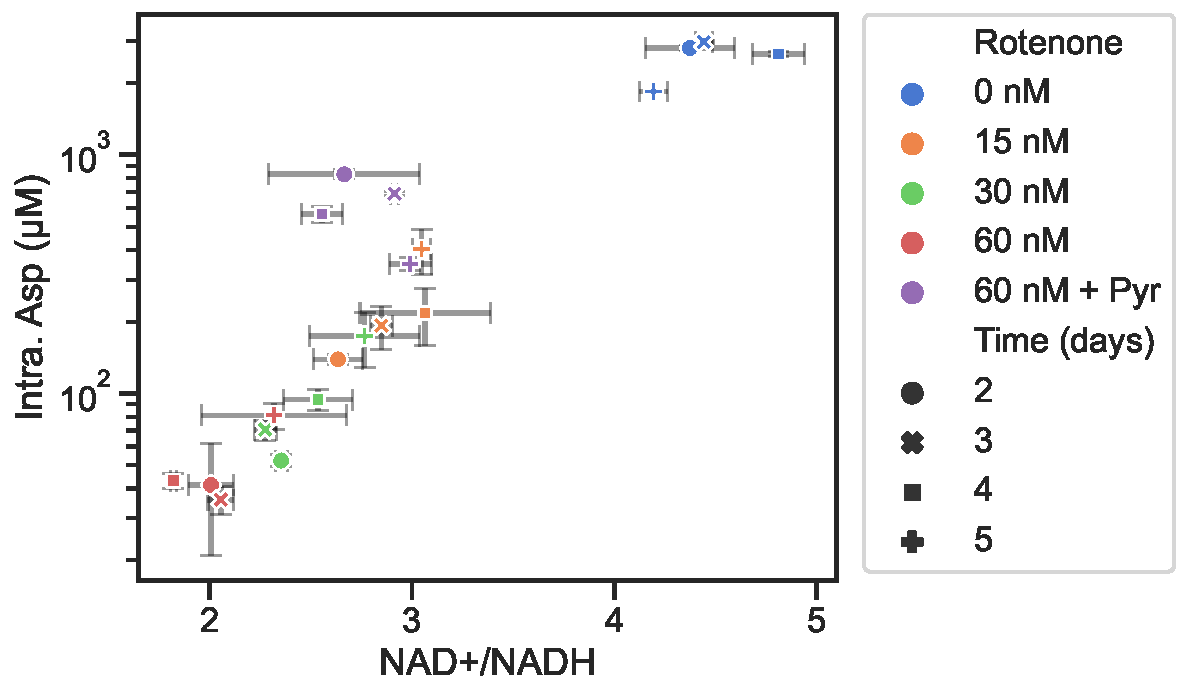
\includegraphics[width=0.6\textwidth]{figures/chap2/NAD-NADH-Asp_rep1-2.pdf}
    \caption[Aspartate and \NAD{}/NADH ratios are correlated.]{
    Correlation between the intracellular aspartate concentration and the \NAD{}/NADH ratio for data in figure \ref{fig:ch2:NAD_Asp_time}.
    }
    \label{fig:ch2:NAD_Asp_corr}
\end{figure}




\subsection{Quantifying the metabolic fates of aspartate}
The relevant metabolic fates of aspartate are: protein, arginine, asparagine pyrimidines and purines.
It is desirable to know the consumption flux of each aspartate fate as a way of ranking their importance during aspartate limitation.
To achieve this, first amino acid uptake and release was determined for wildtype (WT) 143B cells and its double knockout of the aspartate synthesis genes glutamic oxalacetic transaminases 1 and 2 (GOT DKO) (figure \ref{fig:ch2:flux_143wt_dko}).
The GOT DKO cells have abolished aspartate synthesis, relying on aspartate import via. the SLC1A3 transporter and thus total aspartate consumption can be determine.
It was observed that highly consumed amino acids like glutamine have high uptake flux while rare amino acids like tryptophan like have low uptake, in accordance with previous measurements \cite{Hosios2016-us}.
Permeable amino acids, not present in DMEM like asparagine and proline, are released.
In this experiment, isotopically labelled asparagine was added to the media to quantify its uptake and at the final timepoint intracellular metabolites were extracted to determine the ratio of labelled to unlabelled asparagine inside the cells.
With the flux measurements for unlabelled asparagine release and labelled asparagine uptake, and the intracellular labelling ratio, the other asparagine fluxes could be solved by application of flux conservation (figure \ref{fig:ch2:asn_Jprot}; see methods for details).

Asparagine efflux must be calculated as an initial value because progressive accumulation of asparagine in the media will lead to lower efflux over time.
Thus calculated, the initial efflux of asparagine is close to 2.5 mM/h while asparagine consumption by protein synthesis is 1.5-2 mM/h (figure \ref{fig:ch2:Asn_flux}).
The measured efflux is in good agreement with asparagine efflux measured in GOT DKO cells with did not receive isotopically labelled asparagine \ref{fig:ch2:flux_143dko}).

\begin{figure}
     \centering
     \begin{subfigure}[b]{0.75\textwidth}
         \centering
         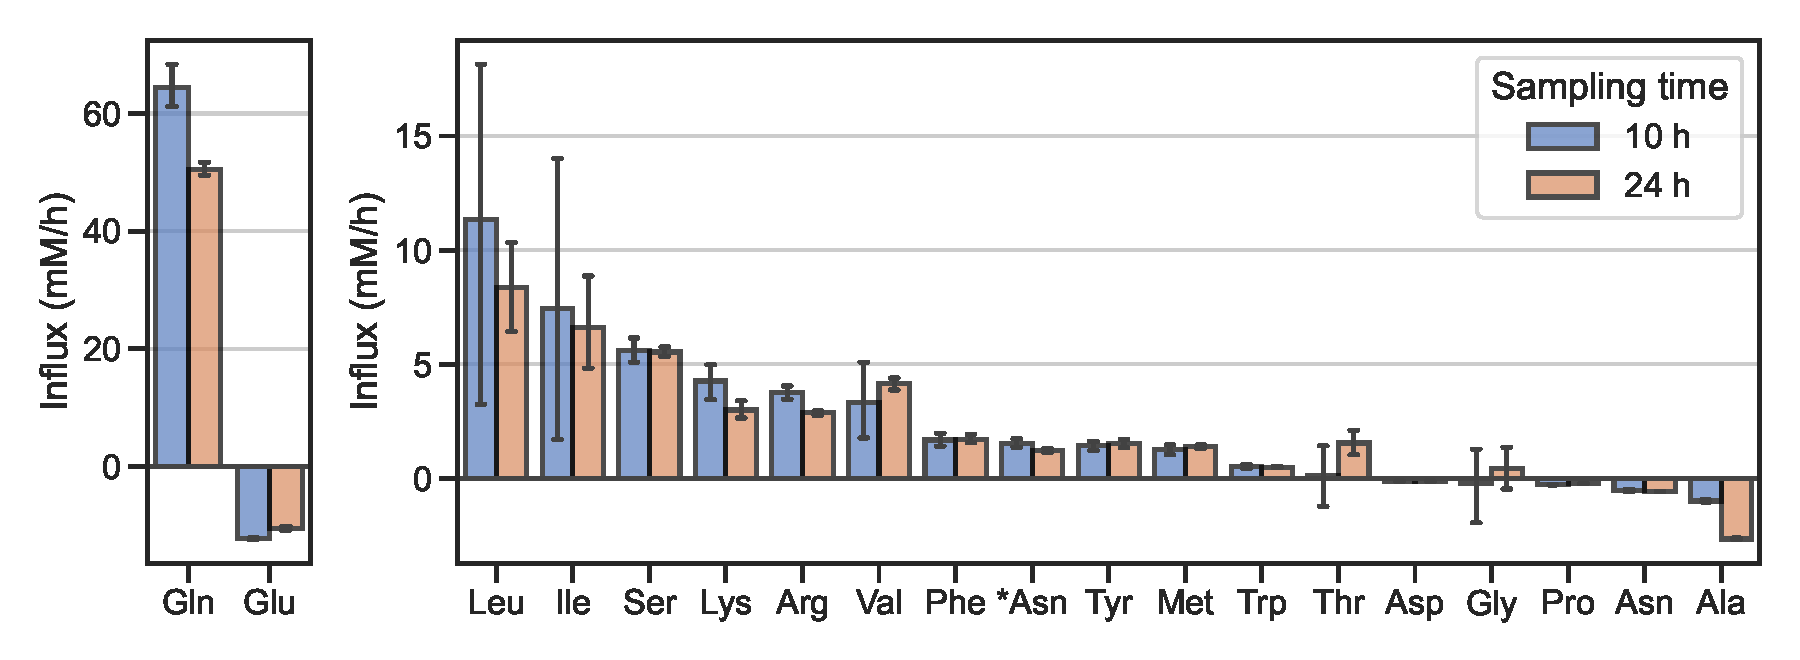
\includegraphics[width=\textwidth]{figures/chap2/flux_143wt.pdf}
         \caption{Media uptake, 143B WT}
         \label{fig:ch2:flux_143wt}
     \end{subfigure}
     \begin{subfigure}[b]{0.75\textwidth}
         \centering
         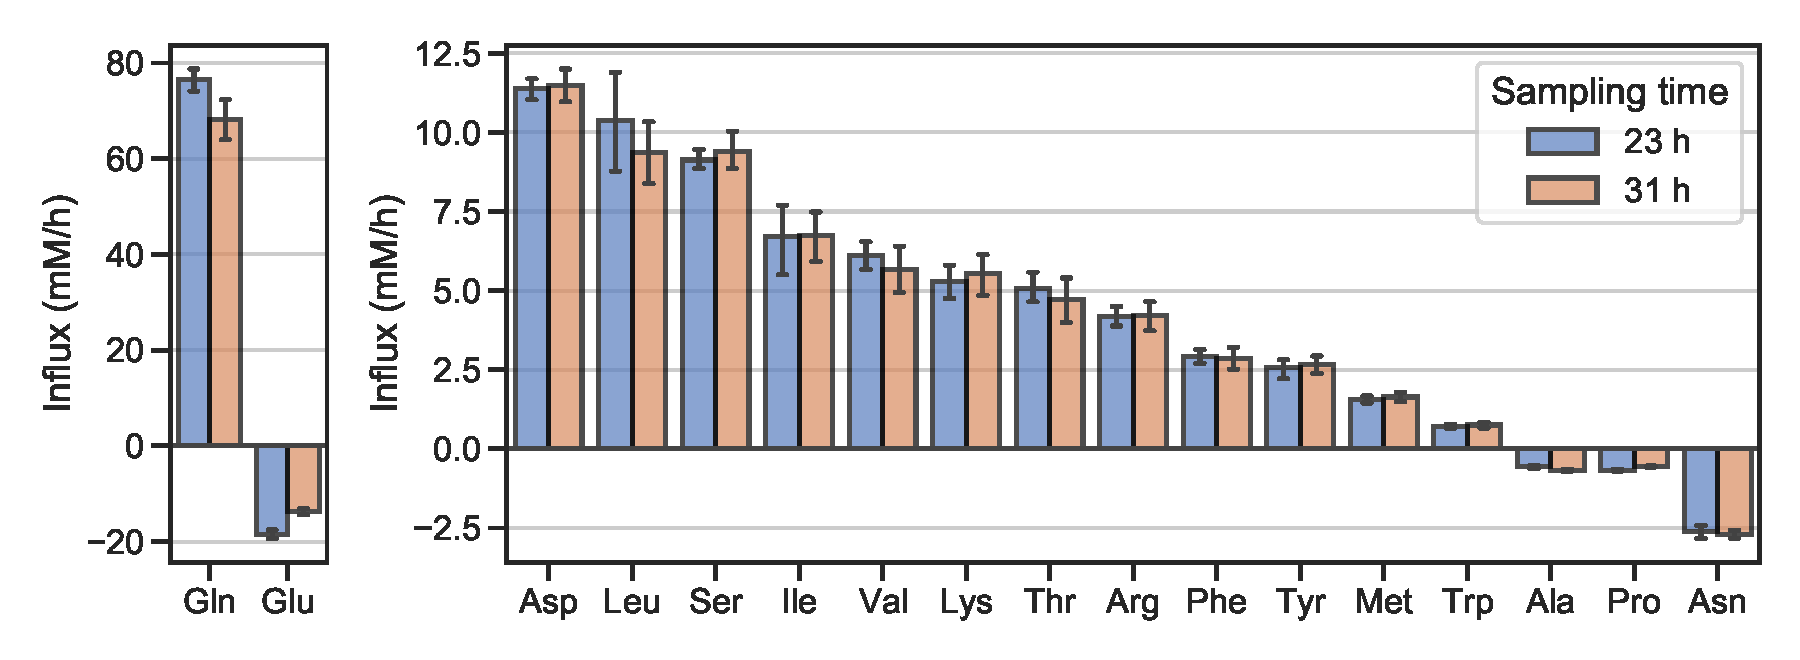
\includegraphics[width=\textwidth]{figures/chap2/flux_143dko.pdf}
         \caption{Media uptake, 143B GOT DKO}
         \label{fig:ch2:flux_143dko}
     \end{subfigure}
        \caption[Media amino acid uptake.]{
        Amino acid influx/efflux from DMEM media.
        For 143B WT in (a), media was spiked with U-\hCi{} Asn (*Asn in the plot) to measure asparagine uptake.
        For 143B GOT DKO in (b), cells expressing Glu/Asp transporter SLC1A3, media was spiked with 500 µM aspartate to measure its uptake.
        }
        \label{fig:ch2:flux_143wt_dko}
\end{figure}

\begin{figure}[ht]
     \centering
     \hspace{0.1\textwidth}
     \begin{subfigure}[b]{0.35\textwidth}
         \centering
         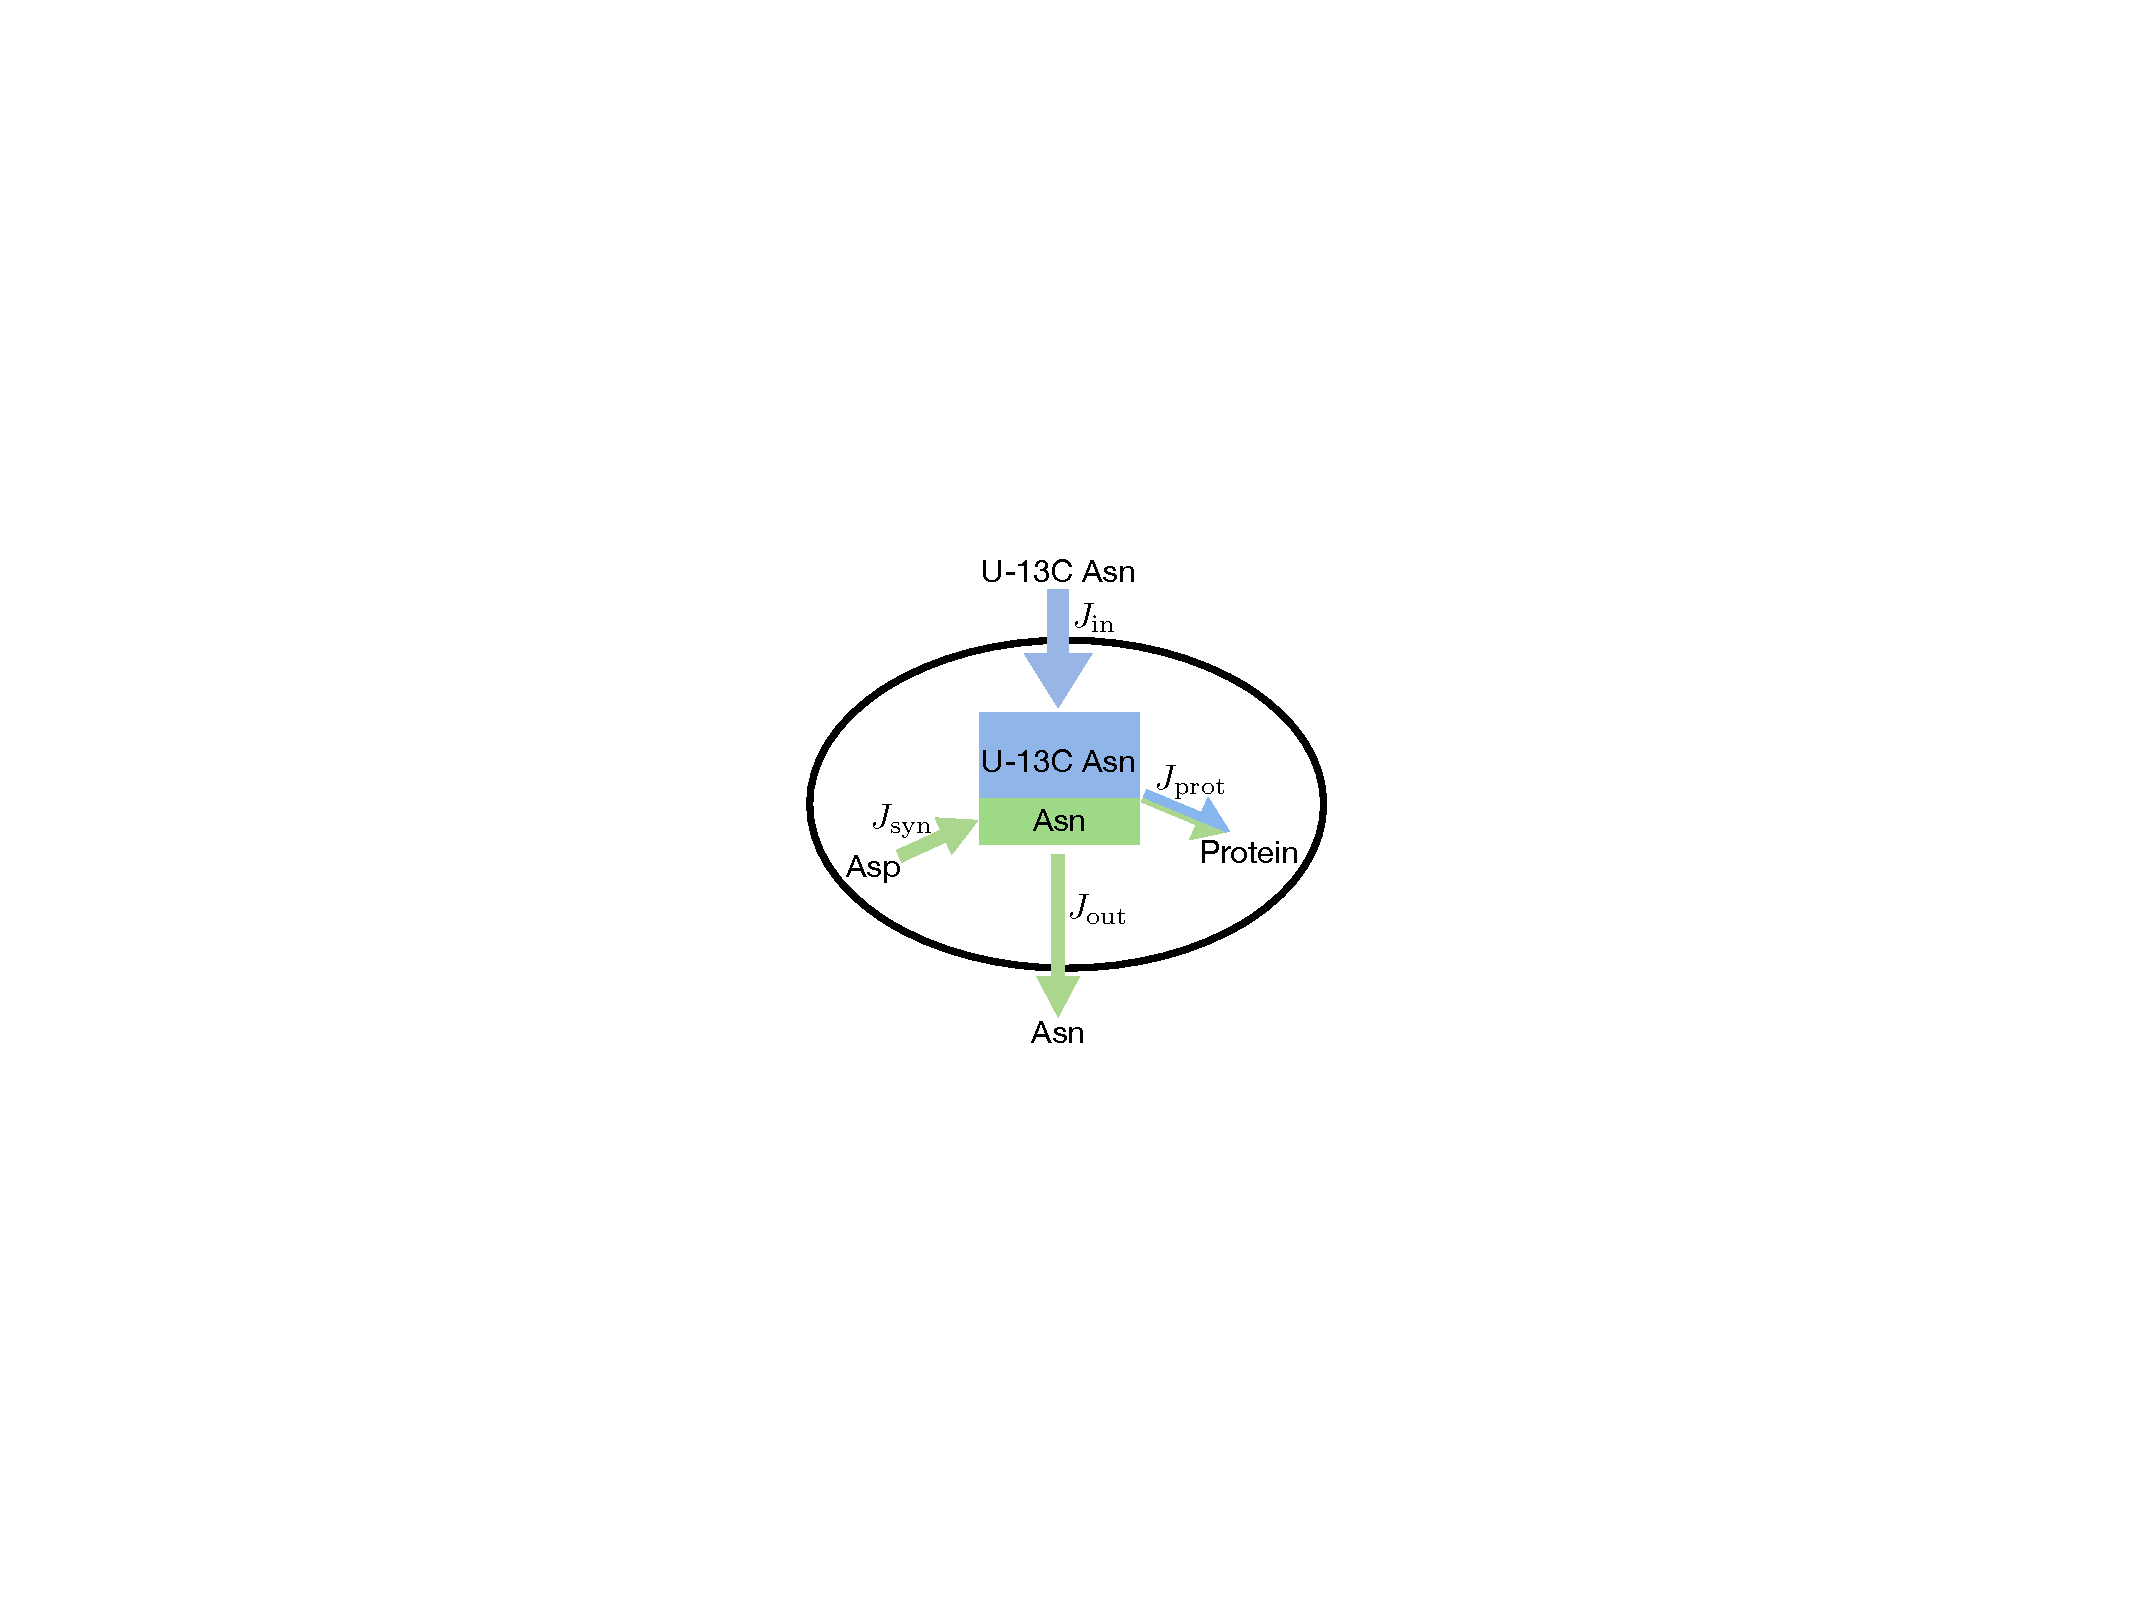
\includegraphics[width=\textwidth]{figures/chap2/asn_Jprot.pdf}
         \caption{Flux diagram}
         \label{fig:ch2:asn_Jprot}
     \end{subfigure}
     \hfill
     \begin{subfigure}[b]{0.4\textwidth}
         \centering
         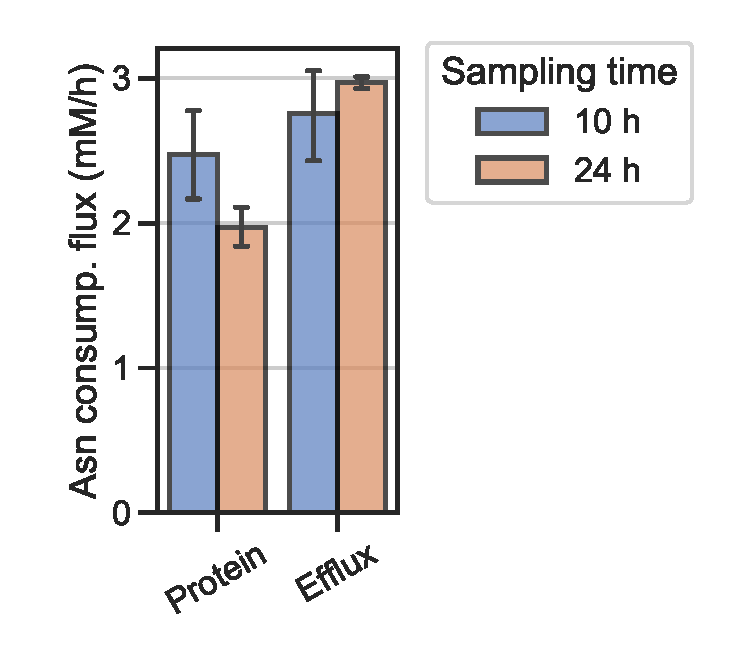
\includegraphics[width=\textwidth]{figures/chap2/Asn_flux.pdf}
         \caption{Asn consumption flux}
         \label{fig:ch2:Asn_flux}
     \end{subfigure}
     \hspace{0.1\textwidth}
        \caption[Asparagine consumption fluxes.]{
        (a) Diagram of asparagine fluxes in a cell.
        Net influx of U-\hCi{} labelled Asn ($\Flin$), net efflux of unlabelled Asn ($\Flout$), net deposition of Asn into protein ($\Flprot$) and Asn synthesis from Asp ($\Flsyn$).
        Unlabelled metabolites symbolized by green and U-\hCi{} labelling symbolized by blue.
        (b) Measured asparagine consumption fluxes in 143B cells using the media uptake data from figure \ref{fig:ch2:flux_143wt}.
        Asn is consumed into protein synthesis (Protein) and leaked into the media (Efflux).
        Efflux is calculated as the initial rate i.e. assuming no Asn is provided in the media.
        }
\end{figure}




To determine aspartate consumption by protein and pyrimidine synthesis, 143B and H1299 cells were hydrolyzed to measure all aspartate, asparagine and arginine bound in protein and all pyrimidines bound in DNA and RNA (figure \ref{fig:ch2:ah_cell_comp}).
Both cell lines show similar total amino acid concentrations, with 143B cells appearing slightly denser than H1299.
Since asparagine and glutamine are entirely deaminated to aspartate and glutamate during acid hydrolysis (appendix figure \ref{fig:app_ch2:AA_acid_hydrolysis_stability}) the sum of asparagine and aspartate is measured.
Similarly, purines are susceptible to acid hydrolysis and cannot be accurately quantified (appendix figure \ref{fig:app_ch2:nucleobase_hydrolysis_stability}).
Therefore, the total concentration of purines was estimated equal to that of pyrimidines, based on published measurements on rat liver RNA \cite{Lipshitz1960-jw}.

Taken together, the flux of each aspartate fate in 143B cells can be inferred (figure \ref{fig:ch2:asp_fate}).
These fluxes shows that protein synthesis is the biggest consumer of aspartate but also that asparagine efflux is a large sink, dependent on media conditions.
The total aspartate consumption flux in DMEM, i.e. with arginine but without asparagine, is estimated to be 9.9 mM/h.
This is close to the aspartate uptake in 143B GOT DKO cells which was measured at 11.4 mM/h (figure \ref{fig:ch2:flux_143dko}).
The difference can be accounted for by considering that total pyrimidine/purine levels underestimate synthesis flux by discounting recycling (figure appendix \ref{fig:app_ch2:pur_tr_ov}) and because 143B GOT DKO cells maintain a higher intracellular concentration of aspartate due to expression of the SLC1A3 aspartate transporter.

\begin{figure}
    \centering
    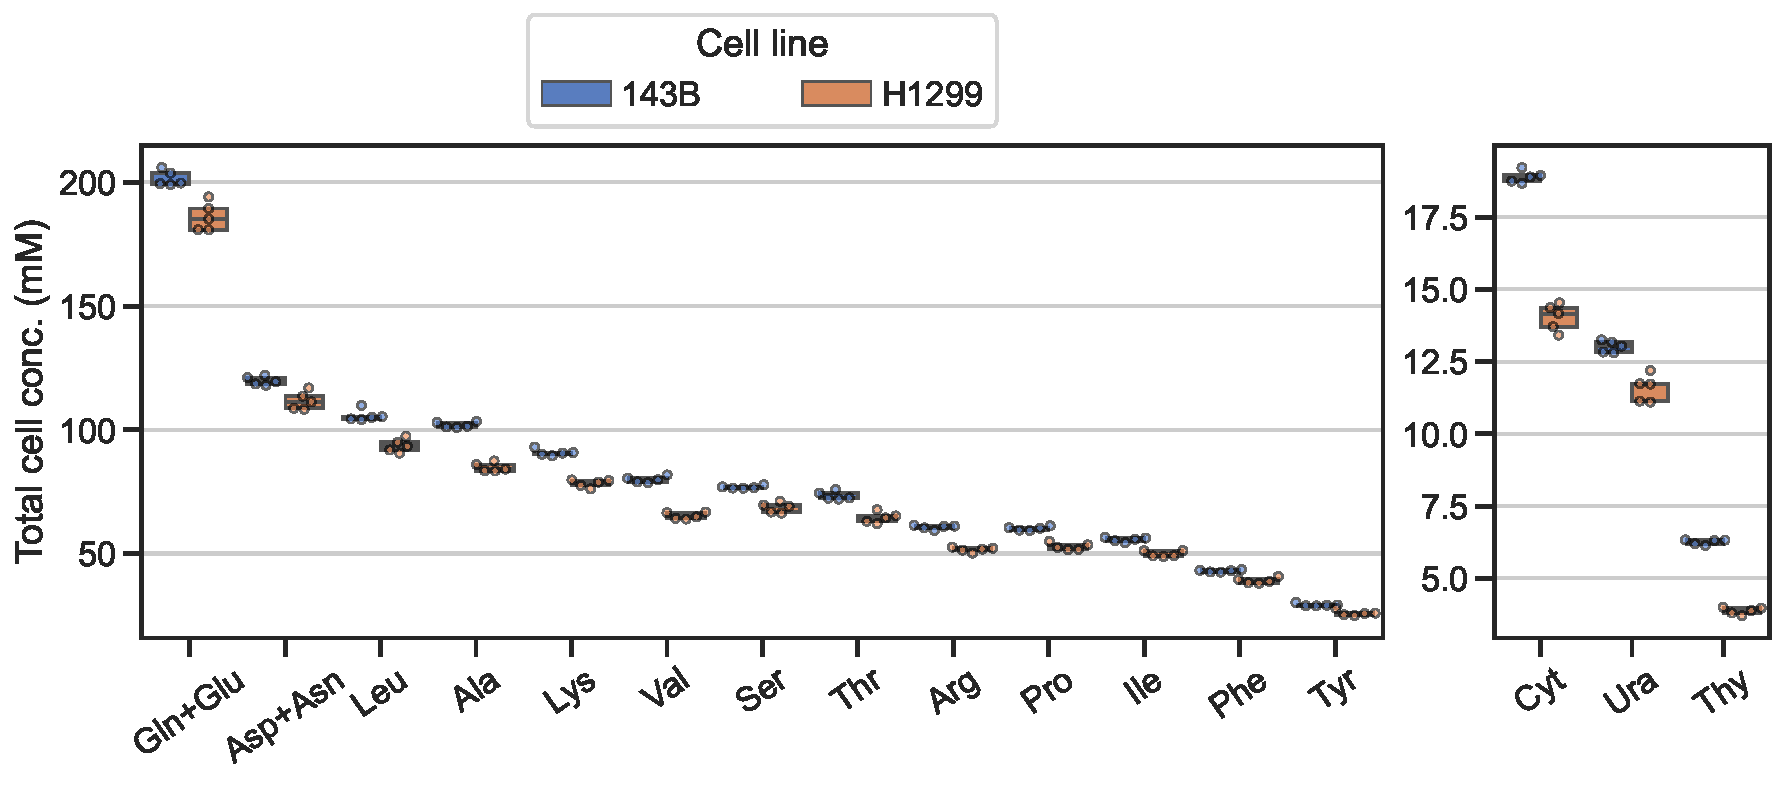
\includegraphics[width=0.80\textwidth]{figures/chap2/ah_cell_comp.pdf}
    \caption[Amino acid and pyrimidine total cell concentration.]{
    Total amino acids and pyrimidines liberated by acid hydrolysis of 143B and H1299 cells, normalized by total cell volume (Total cell conc.).
    Gln and Asn is converted during acid hydrolysis to Glu and Asp, respectively.
    Glycine is not shown because it is also produced from purine hydrolysis \cite{Markham1949-qy}.
    }
    \label{fig:ch2:ah_cell_comp}
\end{figure}

\begin{figure}[ht]
    \centering
    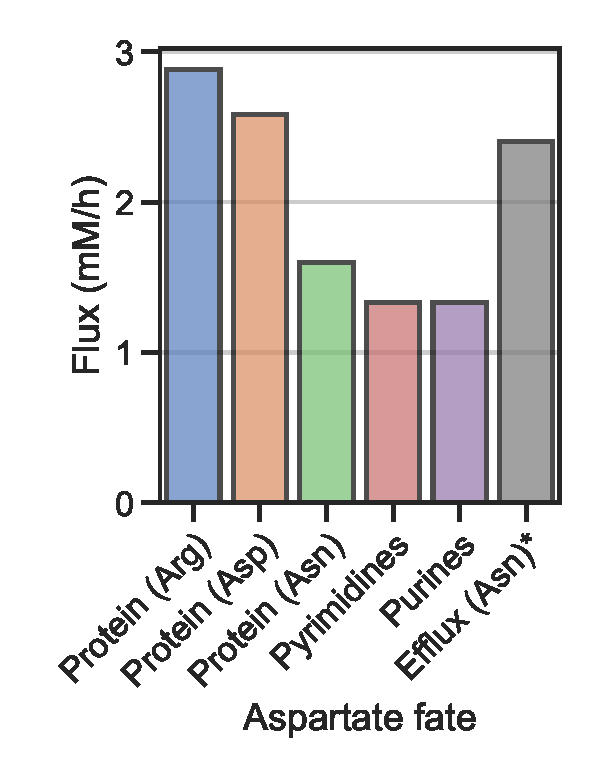
\includegraphics[width=0.36\textwidth]{figures/chap2/asp_fate.pdf}
    \caption[Relative consumption towards each fate of aspartate.]{
    Relative consumption towards each fate of aspartate in 143B cells, estimated using best estimates from figure \ref{fig:ch2:Asn_flux} and \ref{fig:ch2:ah_cell_comp}.
    Synthesis of purines was assumed equal to pyrimidines and thus aspartate consumption towards purines was estimated 1.5 times the consumption towards pyrimidines to account for two aspartate consumed for AMP and one for GMP (see appendix figure \ref{fig:app_ch2:pur_tr_ov}).
    * Asn efflux is calculated as the initial rate for cells are grown in asparagine free media..
    Blue bars indicate the aspartate fate is a nitrogen donation yielding fumarate, red bars indicate the fate consumes aspartate carbons.
    }
    \label{fig:ch2:asp_fate}
\end{figure}




\subsection{Salvage can fulfill all the non-protein metabolic fates of aspartate}
Media complementation of aspartate fates could be used to identify the mechanisms of aspartate limitation.
Towards this end, isotope tracing was employed to test the ability of cells to divert consumption of aspartate into its metabolic fates by providing a salvageable alternative.
Steady-state tracing was performed with both amide\=/\hNi{} and alpha\=/\hNi{} labelled glutamine to measure the salvage fraction for asparagine, uridine, hypoxanthine, adenine and guanine.
For purines traced with Gln amide\=/\hNi{}, \textit{de novo} synthesis results in GTP with three label incorporations (\hNi{}3) and ATP with two (\hNi{}2), whereas the number of labels decreases if purines are salvaged (figure \ref{fig:ch2:sal_frac_pur}).
The resulting isotopologue distributions for 143B cells show that hypoxanthine salvage is fully substituting \textit{de novo} purine synthesis to the point of IMP.
Interestingly, a similar results is shown for adenine, likely due to deamination and recycling back to IMP (appendix figure \ref{fig:app_ch2:pur_tr_ov}).
Guanine is also salvaged into GTP, but less efficiently at around 20\%, and it is only recycled back into IMP at a small degree apparent by the small changes in ATP labelling.
For H1299, the isotopologue distributions are more complex because of Gln amide to alpha \hNi{} transfer (appendix figure \ref{fig:app_ch2:gln_lab_tranfr}); however, when taking this into account the results are similar to the 143B cells except that guanine is salvaged more efficiently, at higher than 90\%, as well as recycled back into IMP at a higher degree.

These results can be summarized by the relative contribution of each synthesis path into ATP and GTP in cells receiving adenine or guanine, respectively (figure \ref{fig:ch2:sal_frac_pur_paths}).
In summary, for both 143B and H1299, 100 µM adenine is sufficient to displace aspartate consumption for purine synthesis by salvage of adenine directly into AMP and by its recycling into hypoxanthine/IMP.

\begin{figure}
    \centering
    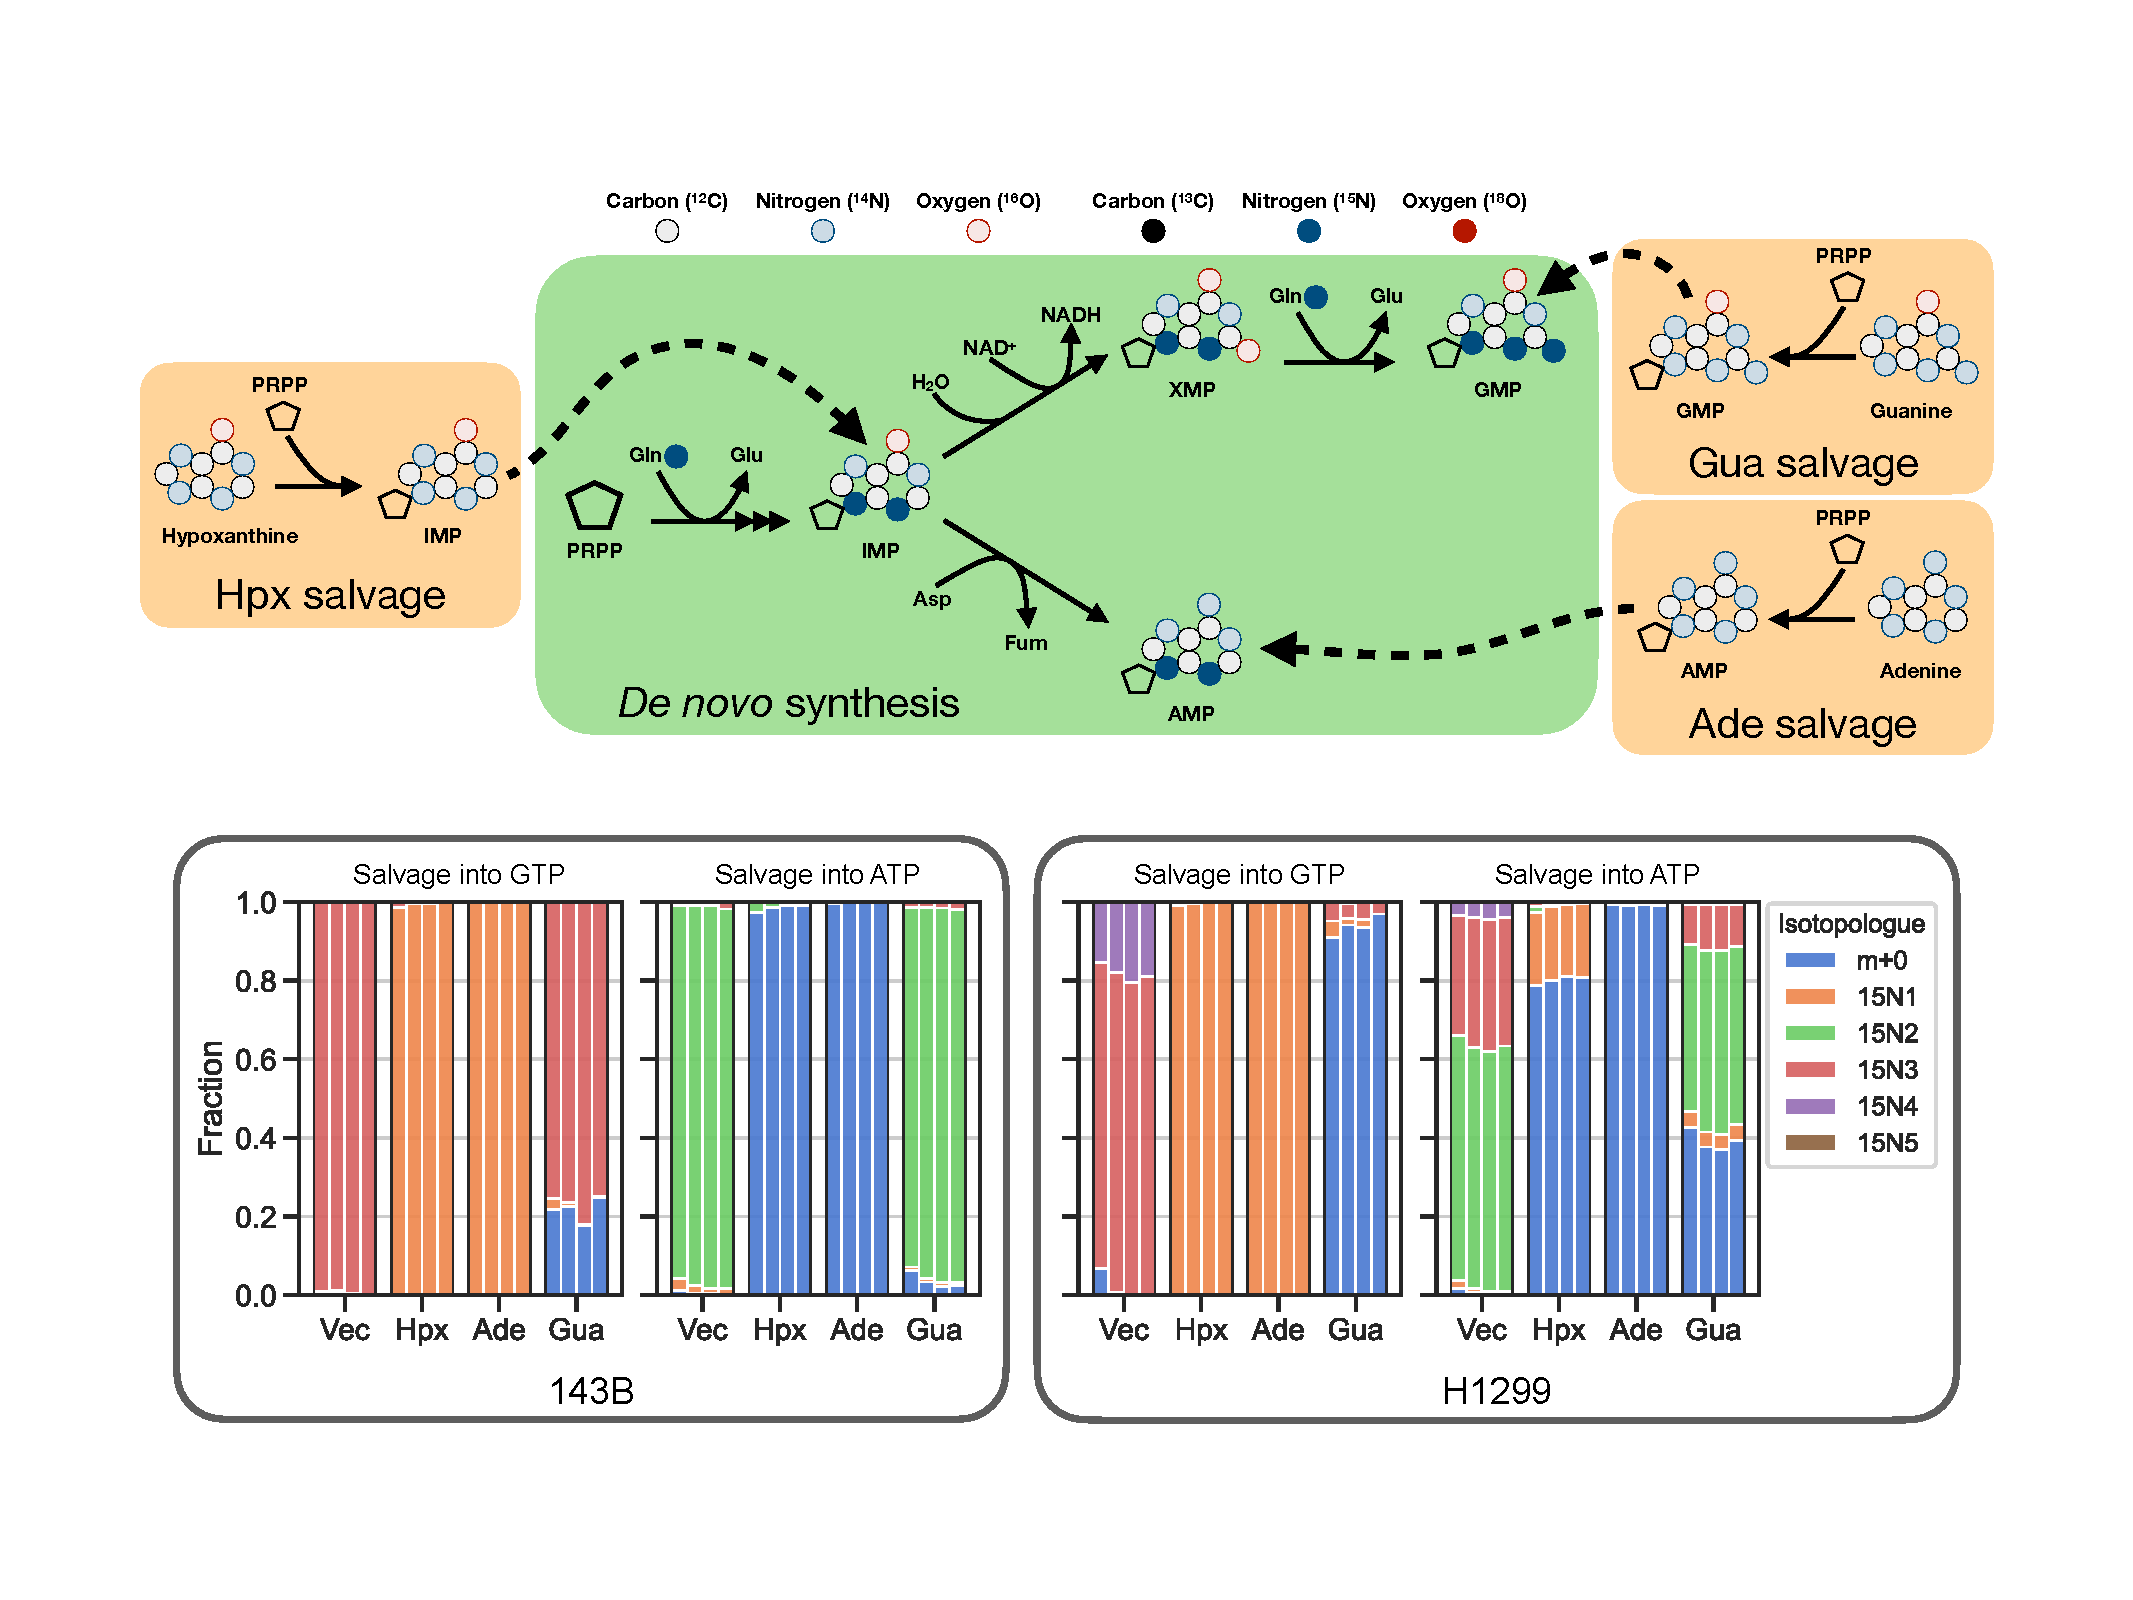
\includegraphics[width=0.98\textwidth]{figures/chap2/sal_frac_pur.pdf}
    \caption[Salvage into purines.]{
    Salvage into purines.
    Top diagram shows Gln amide\=/\hNi{} label incorporation into purines and the resulting changes following salvage of hypoxanthine (Hpx), adenine (Ade) or guanine (Gua).
    Bottom isotopologue distributions show Gln amide\=/\hNi{} label incorporation into GTP and ATP at steady-state for cell lines 143B and H1299 grown in DMEM supplemented with vehicle (Vec) or 100 µM Hpx, Ade or Gua.
    The four replicates are plotted as grouped bars.
    }
    \label{fig:ch2:sal_frac_pur}
\end{figure}

\begin{figure}
    \centering
    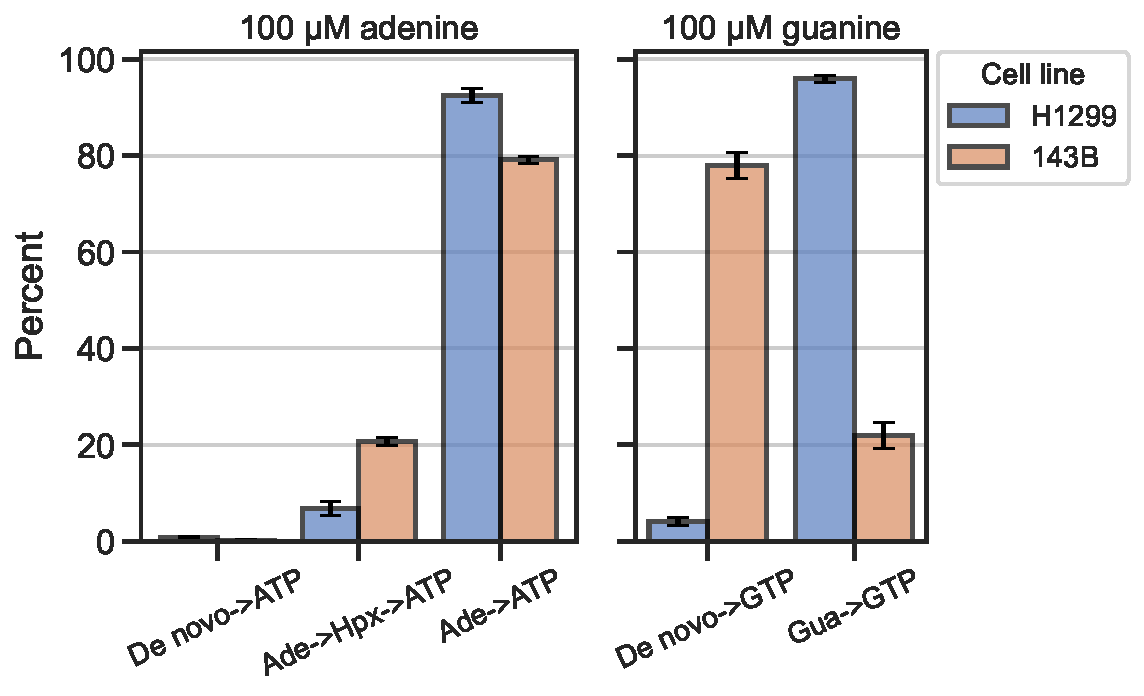
\includegraphics[width=0.6\textwidth]{figures/chap2/sal_frac_pur_paths.pdf}
    \caption[Inferred synthesis paths into purines.]{
    Inferred synthesis paths into ATP and GTP when cells receive 100 µM adenine or guanine, respectively.
    ATP and GTP are either derived from \textit{de novo} synthesis or salvage.
    ATP can be salvaged from adenine directly or through hypoxanthine/IMP as a product of adenine deamination.
    }
    \label{fig:ch2:sal_frac_pur_paths}
\end{figure}




Salvage of asparagine and pyrimidines can also be measured using Gln amide\=/\hNi{} tracing.
Asparagine synthesis leads to one label incorporation (15N1) and thus the salvage fraction can be measured by comparing the abundance of unlabelled and 15N1 labelled intracellular asparagine (figure \ref{fig:ch2:sal_frac_pyr-asn}).
Gln amide to alpha \hNi{} transfer in H1299 causes asparagine to be doubly labelled from both glutamine and partially from aspartate.
Consistent with the high permeability of asparagine \cite{Sullivan2018-gz}, its salvage fraction is high in both 143B and H1299 when provided at 500 µM in the media (figure \ref{fig:ch2:sal_frac_pyr-asn}).
A small fraction of unlabelled asparagine persists which indicates continued synthesis; however, uptake is likely sufficient for cellular demands thus making residual synthesis non-essential.
The labelling pattern for UTP synthesis is similar, with one label incorporation (15N1) and a possible second label in H1299 cell from aspartate due to Gln amide to alpha \hNi{} transfer.
Taking amide to alpha \hNi{} transfer into account, the salvage fraction of 200 µM uridine is around 95\% for both 143B and H1299 (figure \ref{fig:ch2:sal_frac_pyr-asn}).

Taken together, salvage of asparagine and uridine is efficient and using a mixture of adenine, uridine and asparagine should be able to fulfill all the non-protein metabolic fates of aspartate.
In such mixture, concentrations must be chosen to be low enough to be non-toxic but high enough to avoid insufficient salvage and depletion.
This could be achieved using a mix of 500 µM asparagine, 200 µM uridine and 100 µM adenine; however, salvage appear to be efficient even at lower concentrations (appendix figure \ref{fig:app_ch2:sal_frac_conc}).
Finally, aspartate consumption by arginine synthesis was also measured using Gln alpha\=/\hNi{} tracing and found to be non-existing (appendix figure \ref{fig:app_ch2:arg_syn}), as expected given the non-hepatic origin of the cell lines used.

\begin{figure}
    \centering
    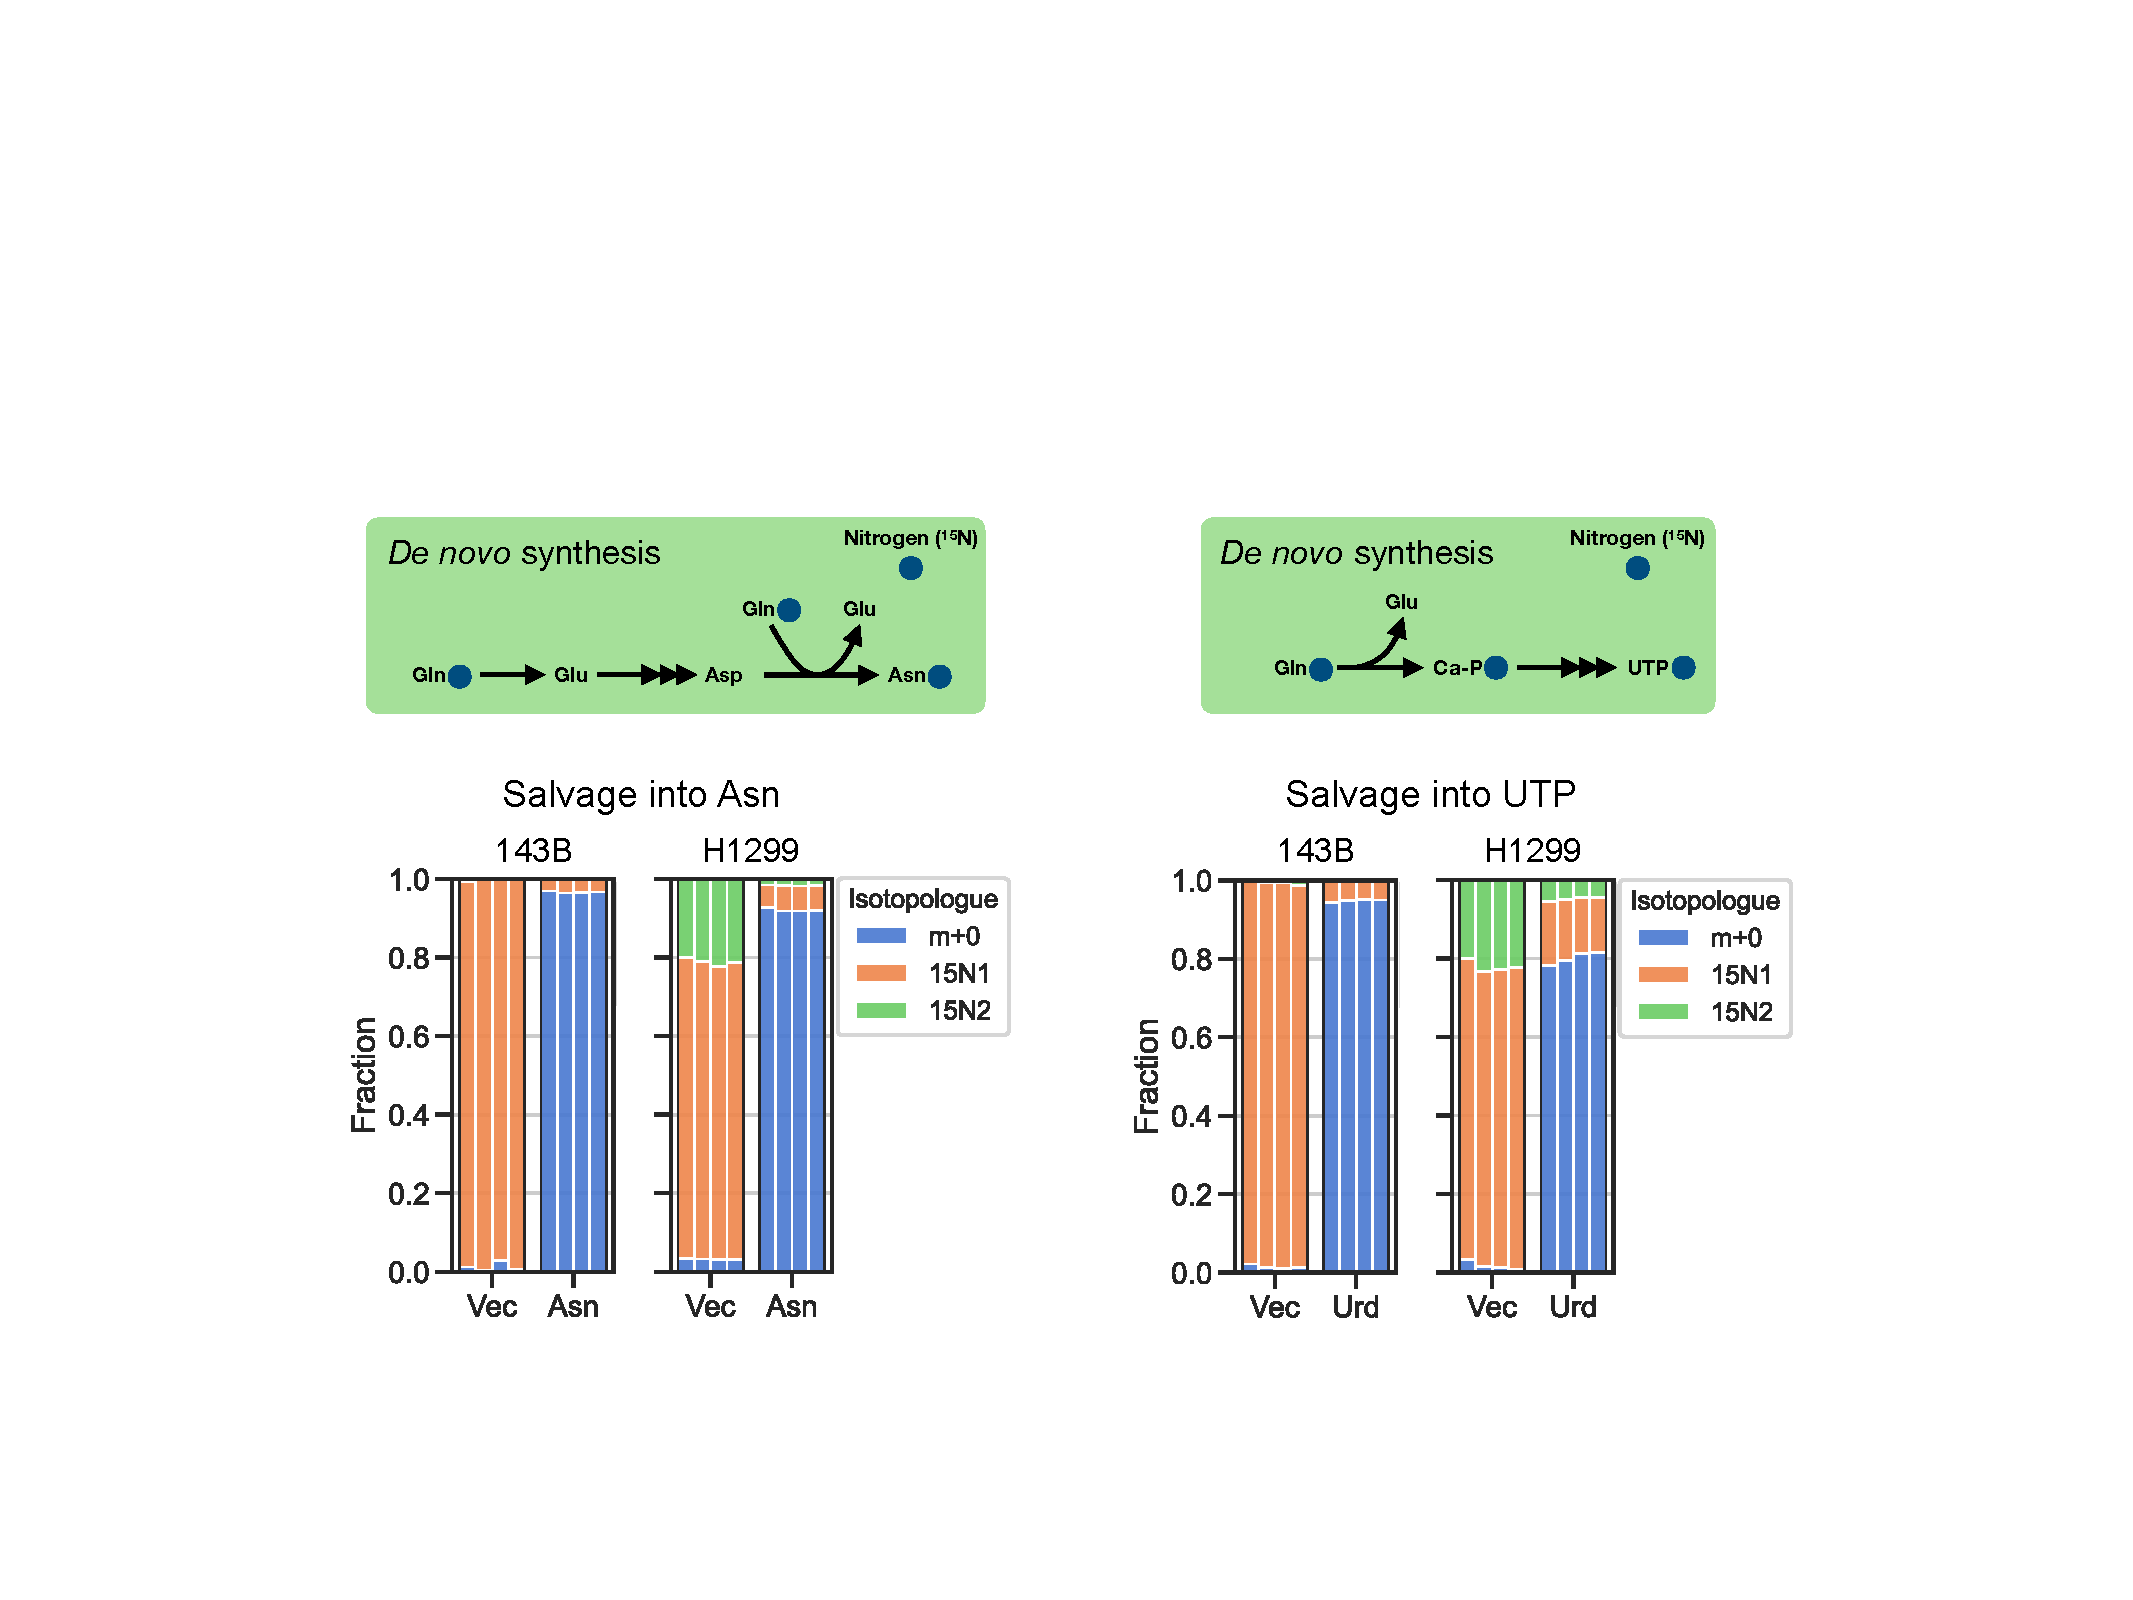
\includegraphics[width=0.8\textwidth]{figures/chap2/sal_frac_pyr-asn.pdf}
    \caption[Salvage into asparagine and pyrimidines.]{
    Salvage into asparagine and pyrimidines.
    Top diagram shows Gln amide\=/\hNi{} label incorporation into asparagine (left) and pyrimidines (right).
    Bottom isotopologue distributions show Gln amide\=/\hNi{} label incorporation into Asn and UTP at steady-state for cell lines 143B and H1299 grown in DMEM supplemented with vehicle (Vec), 500 µM Asn or 200 µM Urd.
    The four replicates are plotted as grouped bars.
    }
    \label{fig:ch2:sal_frac_pyr-asn}
\end{figure}




If any of the metabolic fates of aspartate is the cause of decreased proliferation during aspartate limitation, then adding it back via. salvage could restore proliferation.
In H1299 cells, aspartate limitation was induced using metformin or rotenone and then rescued using the above established routes for salvage (figure \ref{fig:ch2:ETCrescue}).
As a positive control pyruvate shows a robust rescue while each salvaged metabolite shows a small but positive effect of proliferation.
The effect of uridine relative to asparagine is consistent with the relative consumption fluxes (figure \ref{fig:ch2:asp_fate}), suggesting that they exert their effect by diverting aspartate consumption.
It would be tempting to suggest a similar explanation for the rescues made with hypoxanthine and adenine; however, aspartate consumption in purine synthesis is for nitrogen donation and the resulting fumarate can readily be recycled back to aspartate with no net consumption of \NAD{}.
Therefore, the partial rescue of hypoxanthine and adenine is more likely a result of diverting consumption of 10-formyl–THF which is consumed twice during purine synthesis.
This is because 10-formyl–THF production by the folate cycle consumes \NAD{} thereby enhancing the effect of complex I inhibition \cite{Yang2020-fs}.
This explanation is also consistent with results showing that metformin rescue by hypoxanthine and adenine is blunted in serine free media with sodium formate, where the folate cycle no longer consumes \NAD{} (appendix figure \ref{fig:app_ch2:H1299_Met_rescue_noSer}).

\begin{figure}
     \centering
     \begin{subfigure}[b]{0.45\textwidth}
         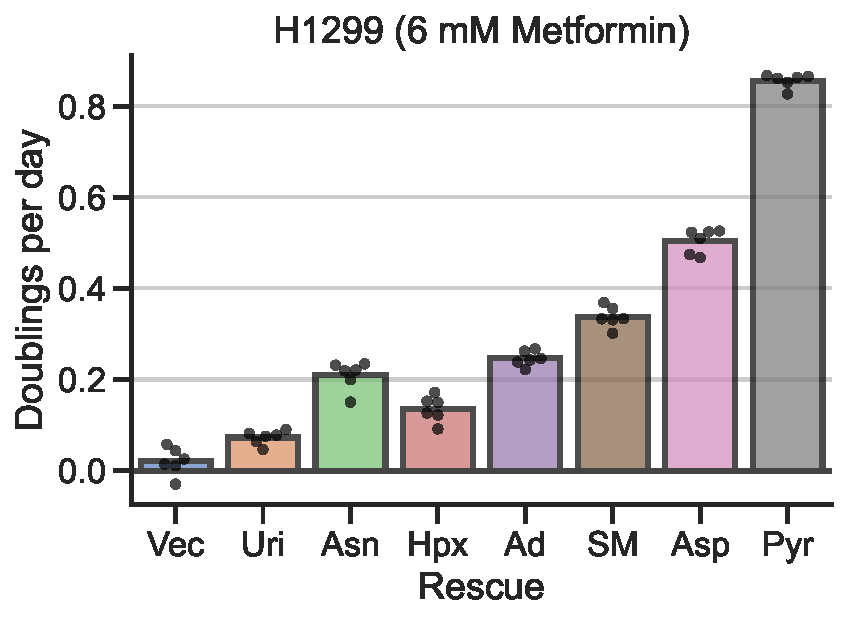
\includegraphics[width=\textwidth]{figures/chap2/H1299_Met_rescue.pdf}
         \caption{}
         \label{fig:ch2:H1299_Met_rescue}
     \end{subfigure}
     \hfill
     \begin{subfigure}[b]{0.45\textwidth}
         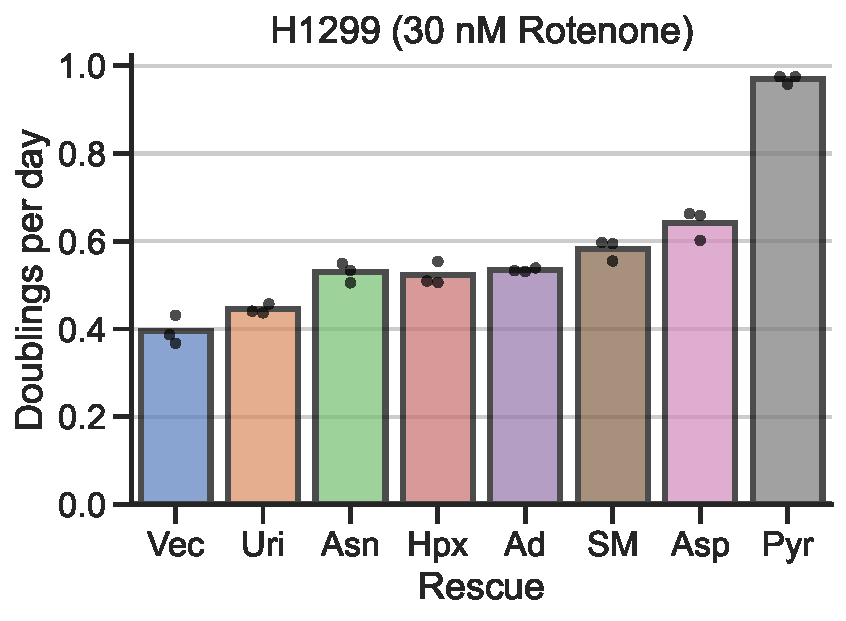
\includegraphics[width=\textwidth]{figures/chap2/H1299_Rot_rescue.pdf}
         \caption{}
         \label{fig:ch2:H1299_Rot_rescue}
     \end{subfigure}
        \caption[Rescuing aspartate limitation with aspartate fates.]{
        Rescuing aspartate limitation with aspartate fates.
        In (a) inducing aspartate limitation with 6 mM metformin and in (b) with 30 nM rotenone.
        Rescuing with vehicle (Vec), 200 µM uridine (Urd), 500 µM asparagine (Asn), 100 µM hypoxanthine (Hpx), 100 µM adenine (Ad), salvage mix (SM), 20 mM aspartate (Asp) or 2 mM pyruvate (Pyr).
        Salvage mix contain: 500 µM asparagine, 200 µM uridine and 100 µM adenine. 
        }
        \label{fig:ch2:ETCrescue}
\end{figure}




\subsection{Proliferation is not controlled by the non-protein metabolic fates of aspartate}
The salvageable fates of aspartate partially rescues proliferation.
Two models can be proposed to explain this:
Model 1, the decrease in proliferation during aspartate limitation is controlled by the one metabolic fate of aspartate which becomes limiting first.
When this fate is salvaged, proliferation is partially restored until a second metabolic fate of aspartate becomes limiting at a lower aspartate level etc.
In this model, providing salvageable metabolites for the metabolic fates of aspartate should partially rescue proliferation and enable cells to maintain proliferation at lower aspartate levels.
Model 2, the decrease in proliferation during aspartate limitation is not controlled by any of the salvageable fates of aspartate.
Thus, provided with salvageable fates of aspartate, proliferation is partially restored only by diverting aspartate consumption, but it does not allow proliferation at lower aspartate levels.
In model 1, when cells are provided with a ``salvage mix'' to fulfill the metabolic fates of aspartate, the aspartate to proliferation relationship must shift leftwards to reflect proliferation at lower aspartate concentrations.
For model 2, the aspartate to proliferation relationship should remain, or at least not shift leftwards.
When performing this experiment in H1299 cells the aspartate to proliferation relationship does not shift leftwards, but slightly rightwards, upon addition of salvage mix (figure \ref{fig:ch2:H1299_Rot_Asp_vs_prlfr}).
The reason for the rightwards shift is unknown; however, assuming that tRNA\textsuperscript{Asp} aminoacylation is not limiting, the results rule out model 1.
It is concluded that proliferation is not controlled by the non-protein metabolic fates of aspartate.

Interestingly, when cells are supplied with salvage mix, the intracellular aspartate level at 50\% proliferation is stable between 380-570 µM across different complex I inhibitors and cell lines (appendix section \ref{sec:ch2:app:asp_prlfr}).
In this condition, only aspartate consumption towards protein synthesis should be required and thus this concentration is surprisingly high considering that aspartate-tRNA ligase has a K\textsubscript{M} for aspartate between 16 and 29 µM \cite{Bour2009-fx, Escalante1993-jy, Messmer2009-xm}.

\begin{figure}
    \centering
    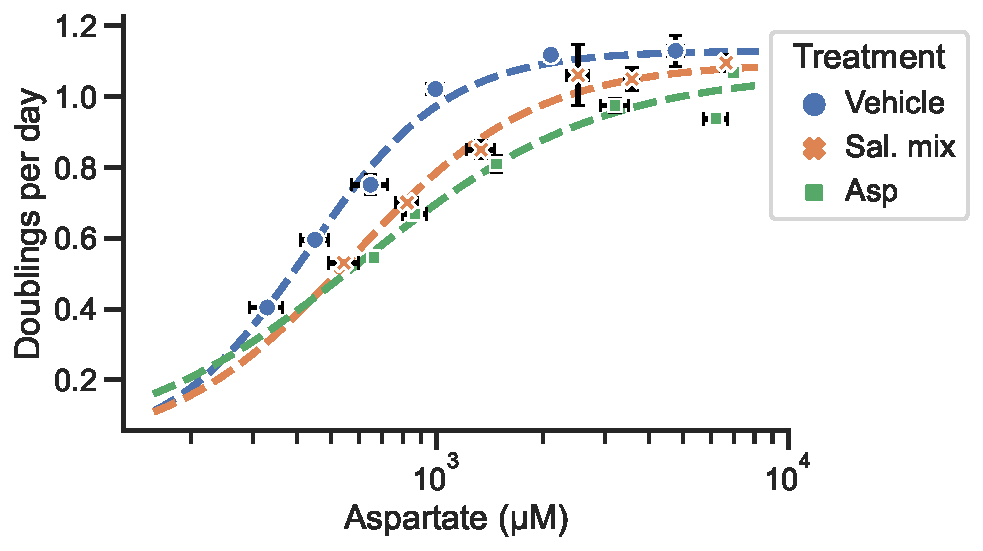
\includegraphics[width=0.7\textwidth]{figures/chap2/H1299_Rot_Asp_vs_prlfr_noPyr.pdf}
    \caption[H1299 rotenone titration aspartate to proliferation.]{
    Aspartate to proliferation relationship for H1299 using rotenone to induce aspartate limitation.
    Aspartate concentration at 50\% proliferation is 430, 570 and 610 µM for Vehicle, Sal. mix and Asp treatments, respectively.
    Condition with salvage mix (Sal. mix) contains: 1 mM asparagine/uridine, 0.5 mM hypoxanthine, 20 µM adenine and 10 µM adenosine.
    }
    \label{fig:ch2:H1299_Rot_Asp_vs_prlfr}
\end{figure}




\subsection{Depleted tRNA charge is not required for aspartate limitation}
None of the salvageable fates of aspartate could relax the aspartate to proliferation relationship, but it remains to be tested if proliferation is limited by protein synthesis directly through uncharged tRNA\textsuperscript{Asp}.
This possibility was tested on H1299 and 143B cells, treated with inhibitors of electron chain complexes I, II, III and V that are known to causes aspartate limitation \cite{Sullivan2015-xf, Hart2023-gp}.
tRNA charge was determined at steady-state using tRNA-seq (see chapter \ref{chap5}) and inhibitors were used at concentrations that result in very little or no proliferation.
The resulting tRNA charges show that some inhibitors do indeed cause a decrease in charge, for example antimycin has a strong effect on tRNA charge in 143B cells (figure \ref{fig:ch2:tRNA:H1299_143B_ETCinhib}).
However, since all the inhibitor treated conditions experience strong aspartate limitation, it can be concluded that depleted tRNA charge is not a defining feature.
This is clear for H1299 cells treated rotenone, which at 100 nM should have proliferation close to zero (appendix figure \ref{fig:app_ch2:H1299_Rot_Rot_vs_prlfr}), but no substantial decrease in tRNA charge is observed.
Most inhibitor induced decreases in tRNA charge appear to happen only for mitochondrial tRNAs.
This also does not support uncharged tRNA being the driver of aspartate limitation because aspartate limited rho0 cells, devoid of any mitochondrial tRNAs, can still be rescued by aspartate \cite{Birsoy2015-pg}.
The possibility of a transient decrease in tRNA charge was also tested, but it appears that tRNA charge decreases monotonically over time after inhibitor treatment (appendix figure \ref{fig:app_ch2:143B_Anti_time}).

\begin{figure}[!ht]
     \centering
     \begin{subfigure}[b]{0.6\textwidth}
         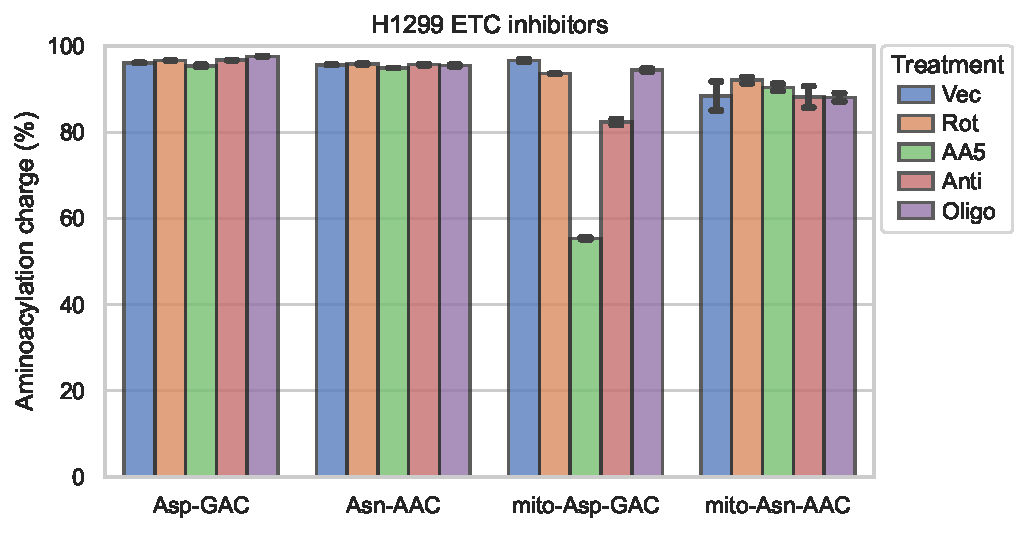
\includegraphics[width=\textwidth]{figures/chap2/H1299_ETCinhib_Asp-Asn.pdf}
     \end{subfigure}
     \begin{subfigure}[b]{0.6\textwidth}
         \vspace{5pt}
         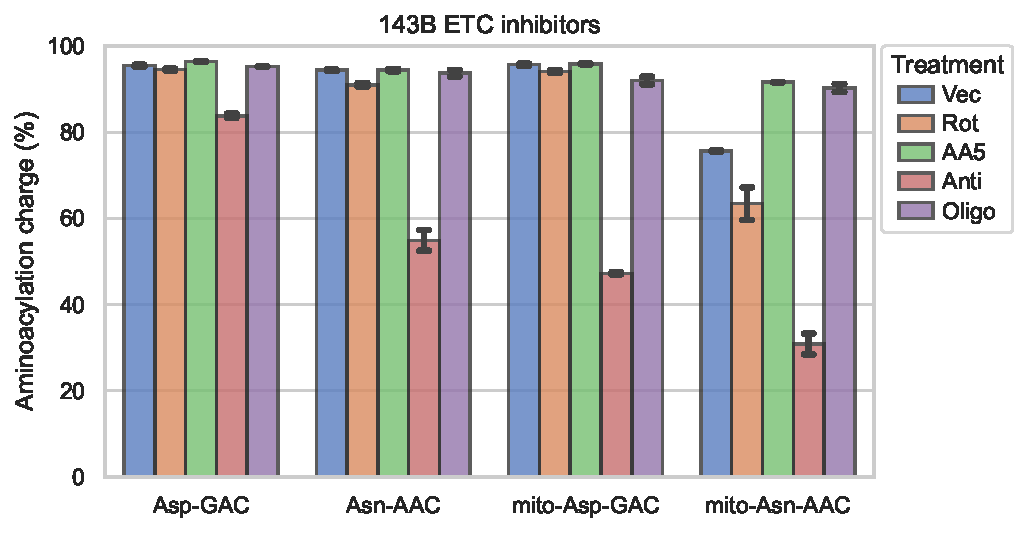
\includegraphics[width=\textwidth]{figures/chap2/143B_ETCinhib_Asp-Asn.pdf}
     \end{subfigure}
     \hfill
        \caption[ETC inhibitor in H1299/143B, effect on tRNA charge.]{
        Steady-state (30 hours) tRNA charge after mitochondrial inhibitor treatment.
        (a) H1299 cells treated with vehicle (Vec), rotenone (Rot; 100 nM), atpenin (AA5; 5 µM), antimycin (Anti; 5 µM) or oligomycin (Oligo; 1 µM).
        (b) 143B cells treated with vehicle (Vec), rotenone (Rot; 50 nM), atpenin (AA5; 5 µM), antimycin (Anti; 0.5 µM) or oligomycin (Oligo; 0.25 µM).
        For all treatments cells were grown in DMEM, without pyruvate, with dialyzed FBS.
        For antimycin and oligomycin treatments, 200 µM uridine was added to the media.
        For the atpenin treatment, 1 mM pyruvate was added to the media.
        }
        \label{fig:ch2:tRNA:H1299_143B_ETCinhib}
\end{figure}




\subsection{Aspartate limitation triggers the integrated stress response through asparagine}
With no evidence supporting that proliferation is controlled by the metabolic fates of aspartate, and the relatively high aspartate concentrations required for cells to maintain 50\% proliferation rate, it seems more likely that a signaling pathway limits proliferation.
The integrated stress response (ISR) is good candidate since it responds to amino acid depletion \cite{Darnell2018-lp} and has more recently been shown activated by mitochondrial inhibitors rotenone, piericidin, antimycin and oligomycin \cite{Guo2020-ia, Mick2020-kf, Condon2021-nz}.
Canonical ISR signals through the kinases GCN2, HRI, PERK and PKR which phosphorylates eIF2alpha to alter translation.
The transcription factor ATF4 is a main target and its abundance increase rapidly following ISR.
Using both standard western blots and an RFP reporter of ATF4, it was found that mitochondrial inhibitors rotenone, metformin and antimycin induce ISR in a dose-responsive way (appendix figures \ref{fig:app_ch2:HT1080_ISR_western} and \ref{fig:app_ch2:atf4_ETCtit}).
The ISR activation could be prevented by supplementation with exogenous electron acceptors pyruvate and alpha-ketobutyrate (figures \ref{fig:ch2:143B_ETCinhib_ATF4rep_low} and \ref{fig:ch2:HT1080_ETCinhib_ATF4rep_high}).
Using complex II inhibitor atpenin to create aspartate limitation, ISR could still be induced without the typical decrease in \NAD{}/NADH ratio (figure \ref{fig:ch2:143B_Atp_ATF4rep}).
Also in this context, using complex I inhibitor rotenone to increase aspartate levels \cite{Hart2023-gp} causes a reduction in ISR.
And lastly, mitochondrial inhibitor induced ISR requires aspartate synthesis \ref{fig:ch2:HT1080_GOT_DKO_ETCinhib_ATF4rep}), as would be expected if ISR is induced by aspartate limitation and not by other effects of mitochondrial inhibition.

In summary, aspartate limitation clearly triggers ISR.
However, unlike aspartate limitation, the ISR induced by rotenone and antimycin could be completely ablated by asparagine supplementation.
This is consistent with a recent report using mouse myoblasts which also found that mitochondrial inhibitor induced ISR could be reversed with asparagine \cite{Mick2020-kf}.
It is also consistent with a rapid drop in intracellular asparagine preceding ATF4 accumulation (figure \ref{fig:ch2:ISR_resc}).

\begin{figure}
     \centering
     \begin{subfigure}[b]{0.49\textwidth}
         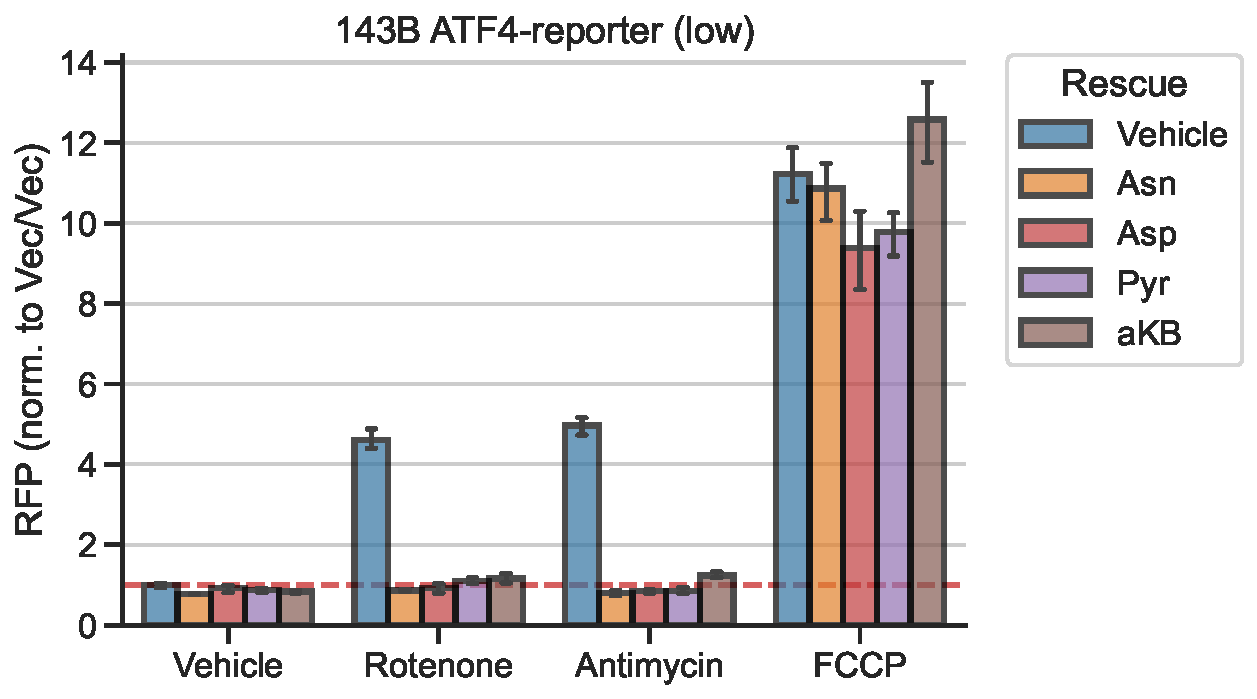
\includegraphics[width=\textwidth]{figures/chap2/143B_ETCinhib_ATF4rep_low.pdf}
         \caption{}
         \label{fig:ch2:143B_ETCinhib_ATF4rep_low}
     \end{subfigure}
     \hfill
     \begin{subfigure}[b]{0.49\textwidth}
         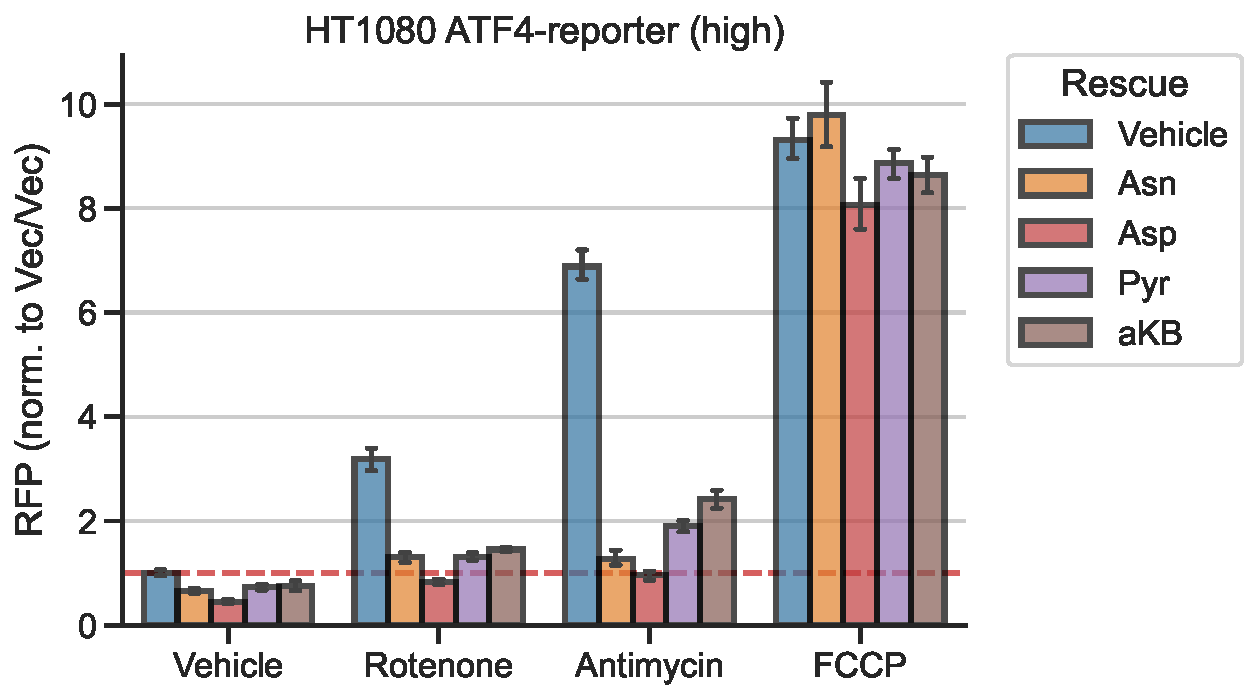
\includegraphics[width=\textwidth]{figures/chap2/HT1080_ETCinhib_ATF4rep_high.pdf}
         \caption{}
         \label{fig:ch2:HT1080_ETCinhib_ATF4rep_high}
     \end{subfigure}
     \hfill
     \begin{subfigure}[b]{0.4\textwidth}
         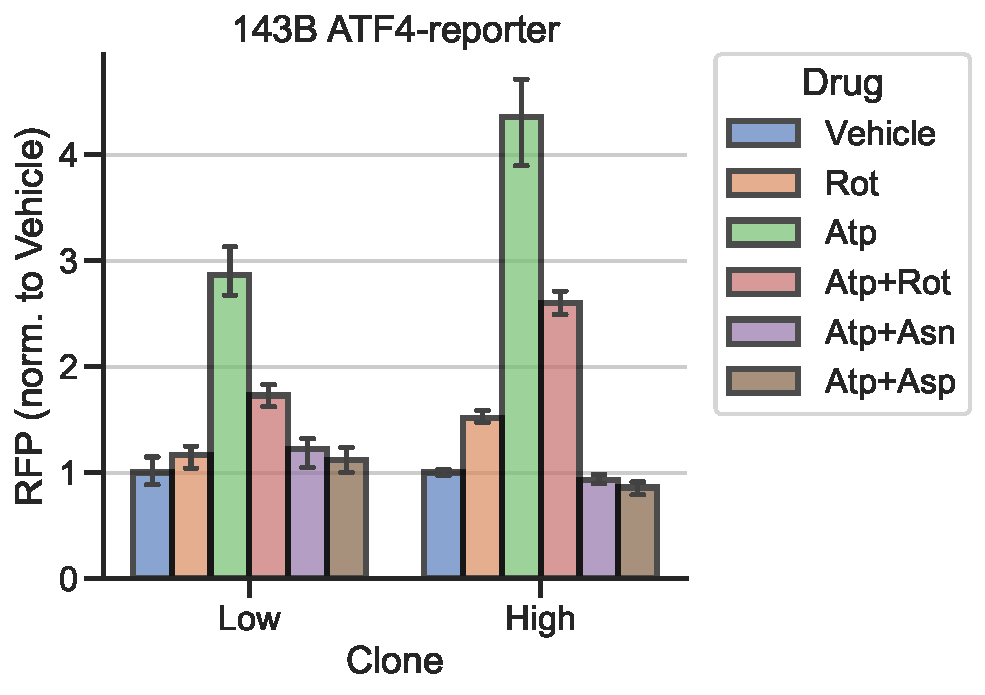
\includegraphics[width=\textwidth]{figures/chap2/143B_Atp_ATF4rep.pdf}
         \caption{}
         \label{fig:ch2:143B_Atp_ATF4rep}
     \end{subfigure}
     \hspace{0.06\textwidth}
     \begin{subfigure}[b]{0.4\textwidth}
         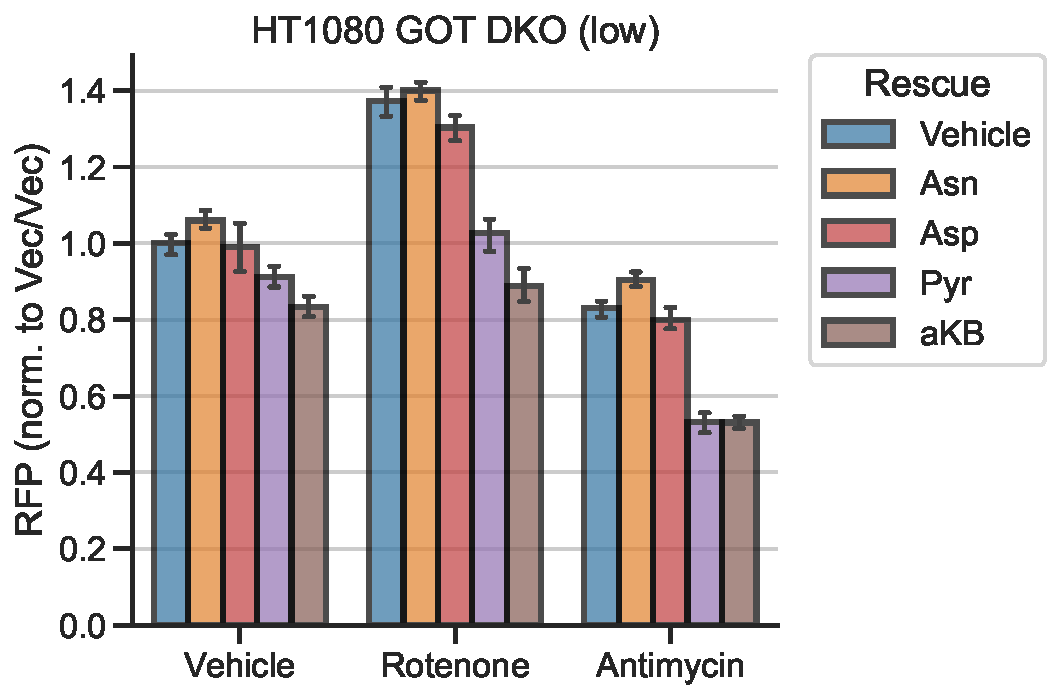
\includegraphics[width=\textwidth]{figures/chap2/HT1080_GOT_DKO_ETCinhib_ATF4rep.pdf}
         \caption{}
         \label{fig:ch2:HT1080_GOT_DKO_ETCinhib_ATF4rep}
     \end{subfigure}
        \caption[Mitochondrial inhibitor induced ATF4 is rescued by Asn.]{
        Mitochondrial inhibitor induced ATF4 reporter expression is prevented by media asparagine.
        (a) and (b), data for two clones with low and high reporter expression at baseline.
        FCCP is a membrane potential uncoupler and used as a positive control.
        (c) Rotenone can partially prevent ATF4 reporter expression induced by atpenin.
        (d) GOT DKO cells are not responding to mitochondrial inhibitors; however, they do respond to aspartate depletion (appendix figure \ref{fig:app_ch2:HT1080_GOT_DKO_Asp_ATF4rep}).
        Similar data for other clones in appendix figure \ref{fig:app_ch2:ISR}.
        }
        \label{fig:ch2:ISR}
\end{figure}

\begin{figure}[ht]
     \centering
     \begin{subfigure}[b]{0.6\textwidth}
         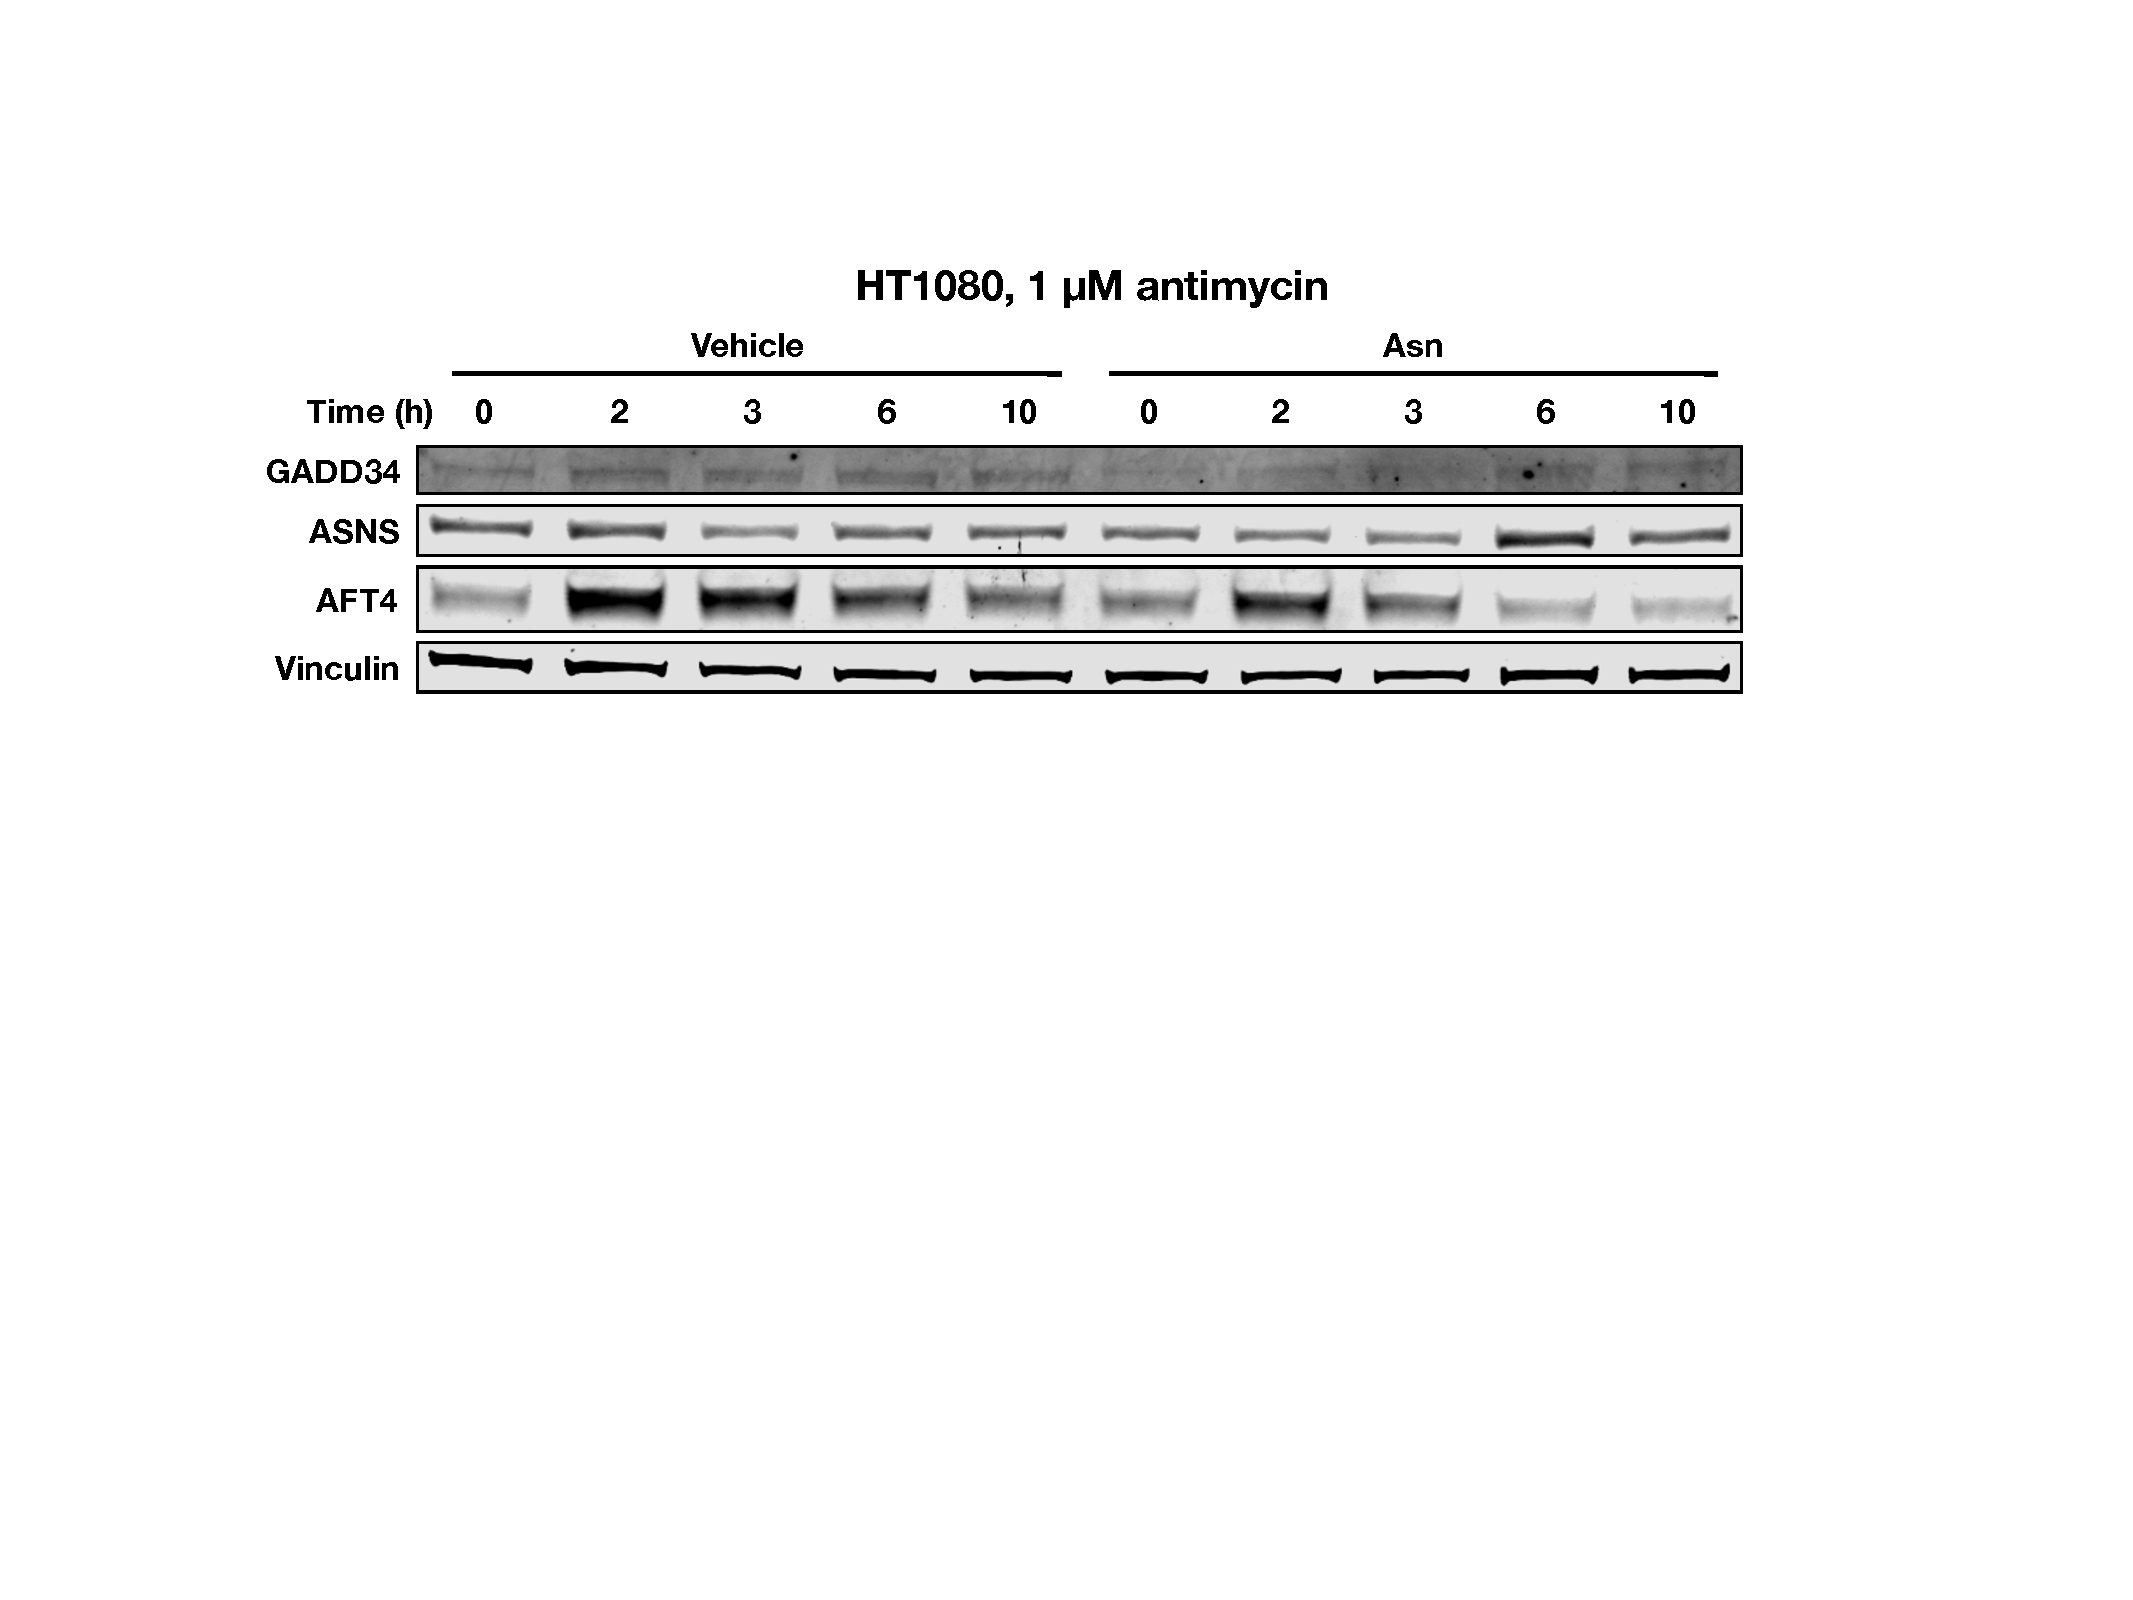
\includegraphics[width=\textwidth]{figures/chap2/HT1080_Anti_ATF4_western.pdf}
         \caption{Antimycin induced ISR}
         \label{fig:ch2:HT1080_Anti_ATF4_western}
     \end{subfigure}
     \hfill
     \begin{subfigure}[b]{0.85\textwidth}
         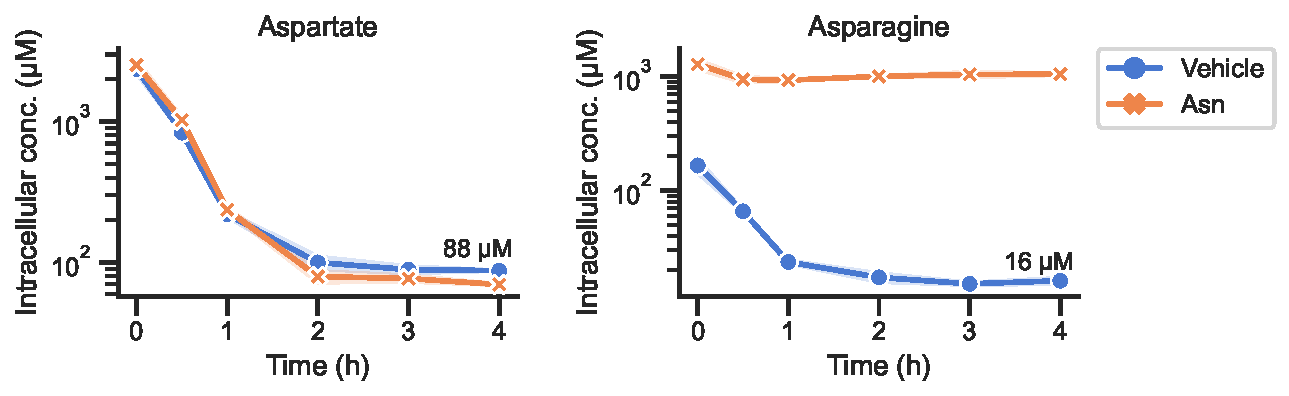
\includegraphics[width=\textwidth]{figures/chap2/HT1080_Anti_Asp_Asn.pdf}
         \caption{Antimycin induced Asp/Asn depletion}
         \label{fig:ch2:HT1080_Anti_Asp_Asn}
     \end{subfigure}
     \hfill
        \caption[Antimycin induced ISR correlates with Asn depletion.]{
        Antimycin induced ISR correlates with Asn depletion in HT1080 WT cells.
        (a) Antimycin (1 µM, media change) induced ATF4 accumulation is partially prevented by media asparagine (100 µM).
        (b) Intracellular Asp/Asn in HT1080 cells grown and treated in parallel with the cells used for (a).
        }
        \label{fig:ch2:ISR_resc}
\end{figure}




\section{Discussion}
Despite the efforts presented in this chapter it is still unclear what causes proliferation decrease during aspartate limitation.
However, the current data highlights several important aspects of aspartate limitation that were not previously known.
First, the aspartate consumption fluxes revealed the importance of asparagine efflux as a larger consumption flux than asparagine consumption by protein synthesis.
This could help explain the relatively large proliferation rescue observed upon asparagine supplementation to complex I inhibited cells in culture and the compounding anti-tumor effect of \textit{in vivo} asparagine depletion using 
asparaginase and complex I inhibitor metformin \cite{Krall2021-mb}.
Second, a strategy was validated for complementation of non-protein metabolic fates of aspartate.
Previously, purine bases have been used for complementation of aspartate limited cells but with no validation that these were consumed and provided at sufficient concentrations \cite{Sullivan2015-xf}.
Third, aspartate to proliferation curves were generated with quantification of intracellular aspartate concentrations at steady-state, as opposed to ion counts after 8 hours of treatment \cite{Gui2016-ca}.
This revealed a surprisingly high intracellular aspartate concentration of 380-570 µM necessary to maintain proliferation rate at 50\% while receiving salvage mix to cover all non-protein metabolic fates of aspartate.
Fourth, for the first time tRNA charge data is presented for cells during aspartate limitation.
In line with the high intracellular aspartate concentrations required for proliferation, uncharged tRNAs do not appear to be required for aspartate limitation.
And lastly, it was shown that while the integrated stress response is turned on upon aspartate limitation it can be ablated with asparagine and thus it is not relevant for aspartate's ability to control proliferation.

So how then does aspartate limit proliferation?
One possibility is nucleotide imbalance, which could occur even when metabolic fates of aspartate are provided through a salvage mix.
The balance of nucleotides has large effects on cell proliferation and imbalance causes suppression of DNA synthesis and limits progression through S phase of the cell cycle \cite{Diehl2022-gm}.
Indeed, aspartate limitation causes a great increase in IMP \cite{Sullivan2015-xf} which could be due to decreased conversion of IMP to AMP by the aspartate consuming enzyme adenylosuccinate synthase.
Complex III inhibition also appear to increase IMP levels as well as increasing the guanine to adenine ratios (GMP/AMP, GDP/ADP and GTP/ATP; appendix figure \ref{fig:app_ch2:HT1080_Anti_metab}), again pointing towards adenylosuccinate synthase.
For human adenylosuccinate synthase the K\textsubscript{M} for aspartate has been reported to be 950 µM \cite{Van_der_Weyden1974-eq}, whereas for other mammals it has been reported between 230 and 1500 µM \cite{Stayton1983-ao}.
This is within the range of intracellular concentrations that causes aspartate limitation and thus nucleotide imbalance should be further explored in the future.




\section{Methods and Materials}
\subsection{Cell culture}
Cell lines were acquired from ATCC (143B, H1299, HT1080) and tested to be free from mycoplasma (MycoProbe, R\&D Systems).
Cells were maintained in Dulbecco’s Modified Eagle’s Medium (DMEM) (Gibco, 50-003-PB) supplemented with 3.7 g/L sodium bicarbonate (Sigma, S6297), 10\% fetal bovine serum (FBS) (Gibco, 26140079) and 1x penicillin-streptomycin solution (Sigma, P4333).
Cells were incubated in a humidified incubator at 37°C with 5\% CO2.


\subsection{Western blots}
Protein lysates were harvested in RIPA buffer (Sigma, R0278) supplemented with Halt protease and phosphatase inhibitor cocktail (Fisher, PI78443) and 5 mM EDTA.
Protein concentration was determined using a BCA assay (Fisher, 23225) using bovine serum albumin (BSA) as a protein standard.
Equal amounts of protein were added to LDS sample buffer (ThermoFisher, B0008) with 5\% 2-Mercaptoethanol (Sigma, M3148), denatured at 95°C for 5 min, loaded onto 4–12\% SDS-polyacrylamide gels (Invitrogen, NW04122BOX) along with a prestained protein ladder (ThermoFisher, 26616) and run 35 min at 180V in MES buffer (ThermoFisher, B000202).
Proteins were dry transferred onto a 0.2 µm nitrocellulose membrane using the iBlot2 device (ThermoFisher, IB21001) with the P0 system setting and associated transfer stacks (Fisher, IB23001).
Membranes were blocked with 5\% bovine serum albumin (Sigma, A4503) in tris-buffered saline with 0.1\% Tween-20 (TBS-T) and incubated at 4°C overnight with the following antibodies:
anti-ATF4 (Cell Signaling, 11815S, 1:500),
anti-ASNS (Cell Signaling, 92479T, 1:1000),
%anti-Phospho-eIF2alpha (Cell Signaling, 3398S, 1:500),
%anti-eIF2alpha (Cell Signaling, 5324S, 1:500),
%anti-Phospho-GCN2 (Cell Signaling, 94668S, 1:500),
%anti-GCN2 (Cell Signaling, 3302S, 1:500),
%anti-OMA1 (Cell Signaling, 95473, 1:1000),
anti-GADD34 (Proteintech, 10449-1-AP, 1:500),
%anti-DARS2 (Proteintech, 13807-1-AP, 1:500),
%anti-HRI (Sigma, HPA016496, 1:1000),
%anti-FLAG (Sigma, F1804; 1:1000),
%anti-SLC1A3 (Genetex, GTX20262; 1:500),
anti-GOT2 (Proteintech, 14800–1-AP, 1:750),
anti-GOT1 (Cell Signaling, 34423 S, 1:1000),
anti-Vinculin (Sigma, SAB4200729; 1:10,000) and anti-Tubulin (Sigma, T6199; 1:10,000).
Membranes were washed with TBS-T and the following secondary antibodies were added in blocking buffer: 800CW Goat anti-Mouse IgG (LiCOR, 926–32210; 1:15,000) and/or 680RD Goat anti-Rabbit IgG (LiCOR, 926–68071; 1:15,000) and incubated for 1 hour.
Membranes were washed with TBS-T, incubated for 10 min in TBS-T, washed in deionized water and imaged on a LiCOR Odyssey Near-Infrared imaging system.


\subsection{Proliferation assays}
Cells were trypsinized (Corning, 25,051 CI), resuspended in seeding media, counted (Beckman Coulter Counter Multisizer 4) and seeded overnight onto 6/12/24 well dishes (Corning, 3516;3513;3524) with an initial seeding density of 10,000 cells/mL and a volume of 4, 2 and 1 mL, respectively.
After overnight incubation, 3–6 wells were counted for a starting cell count at the time of treatment.
Treatment was initiated either by media switch or by spike-in of drug/metabolite from a 20-50x stock.
For both seeding and treatment, experiments were conducted in DMEM without pyruvate (Corning 50–013-PB) supplemented with 3.7 g/L sodium bicarbonate, 10\% dialyzed fetal bovine serum (Sigma, F0392) and 1x penicillin-streptomycin solution, with or without sodium pyruvate (Pyr) (Sigma, P8574),
2-ketobutyric acid (AKB) (Sigma, K401),
aspartate (Asp) (Sigma, A7219),
asparagine (Asn) (Sigma, A7094),
uridine (Urd) (Sigma, U3003), hypoxanthine (Cayman Chemical, 22254),
adenine (Ade) (Sigma, A2786),
guanine (Gua) (Sigma, 51030) or sodium formate (Sigma, 71539) with concentration noted when relevant.
Drug treatments included rotenone (Sigma, R8875),
metformin (Sigma, D150959),
atpenin A5 (Cayman Chemical, 11898; AdipoGen, AG-CN2-0110; Abcam, ab144194; or Enzo Life Sciences, ALX-380–313),
%doxycycline hydrochloride (Sigma, D3447),
antimycin A (Sigma, A8674),
oligomycin A (Sigma, 495455),
%GCN2iB (MedChemExpress, HY-112654),
FCCP (Cayman Chemical, 15218-10),
%UCPH (HelloBio, HB0630),
BAM15 (Cayman Chemical, 17811)
and DMSO vehicle (Sigma, D2650).
Cells were incubated in a humidified incubator at 37°C with 5\% CO2, then counted after 4–6 days.
Proliferation rate was reported as doublings per day and determined using the time and fold count difference between the starting and final counts, assuming a constant proliferation rate throughout the assay.


\subsection{Generation of nuclear RFP cell lines}
Nuclear RFP cell lines were generated using 1e5 transducing units of EF1A-nuclear RFP lentivirus (Cellomics Technology, PLV-10205-50) by spinfection.
Cells were seeded at 50\% confluency on 6 well dishes, lentivirus was added to fresh media with 8 µg/µL polybrene, then added to cells and followed by centrifugation (900g, 90 mins, 30°C).
Two days after infection, cells were sorted for high RFP expression using fluorescence-activated cell sorting (FACS).
High RFP cells were then expanded and single-cell cloned by limiting dilution, plating 0.5 cells/well on a 96 well plate.
Plates were then screened for RFP expression and localization using Incucyte S3 (Sartorius) and a suitable clone chosen, expanded, and used for all subsequent experiments.


% Don't think this is necessary. Did not use Incucyte for proliferation in this chapter
%\subsection{Incucyte measurements}
%Live cell imaging was performed on the Incucyte S3 using the RFP channel with %default exposure time and 20x magnification.
%Cells expressing nuclear RFP was used to estimate cell counts per well by counting the number of nuclear foci in each field of view when scanning in the RFP channel.
%Cell confluency was determined with the phase contrast scans.
%All image analysis was performed using the associated Incucyte software.


\subsection{Lentiviral production and stable cell line generation}
The following plasmids were obtained: pLenti6.3-V5 DEST\_SLC1A3 (DNASU Plasmid Repository) and ATF4 reporter pXG237 (Addgene, 141281).
%pLHCX-gpASNase1 (Addgene, 121526)
%and pDONR221\_EGFP (Addgene, 25899).
%ASNS was cloned by PCR from HEK293T reverse transcribed mRNA.
Genes were first cloned into entry vector pENTR1A (Fisher, A10462) using NEBuilder HiFI DNA Assembly Cloning Kit (New England BioLabs, E2621).
These donor constructs were then used to transfer their insert into destination vectors: pLX304-CMV-Blast (Addgene, 25890) or pLenti-CMV-Hygro (w117-1) (Addgene, 17454 a gift from Eric Campeau \& Paul Kaufman) using LR Clonase II (Fisher, 11791100).
Each plasmid sequence was verified by whole plasmid sequencing (Plasmidsaurus).
Lentivirus was generated by co-transfection of HEK293T cells with destination vector plasmid DNA and the packaging plasmids pMDLg/pRRE (Addgene, 12251), pRSV-Rev, (Addgene, 12253) and pMD2.G (Addgene, 12259) using FuGENE transfection reagent (Fisher, PRE2693) in DMEM (Fisher, MT10017CV) without FBS or penicillin-streptomycin.
The supernatant containing lentiviral particles was filtered through a 0.45 µM membrane (Fisher, 9720514) and was supplemented with 8 µg/µL polybrene (Sigma, TR-1003-G) prior to infection.
For infection, cells were seeded at 50\% confluency in 6 well dishes and centrifuged with lentivirus (900g, 90 mins, 30°C).
After 24 hours the media was replaced with fresh media and after 48 hours cells were treated with either 1 µg/mL blasticidin (Fisher, R21001) or 150 µg/mL hygromycin (Sigma, H7772-1G) and maintained in selection media until all uninfected control cells died.
After selection, cells were expanded and single-cell cloned by limiting dilution, plating 0.5 cells/well using 96 well plates.
These clones were expanded and screened by either western blot or presence of RFP signal using Incucyte S3 (Sartorius) to validate expression.
From this, a single clone was chosen, expanded and used for all subsequent experiments.


\subsection{Generation of knockout cells}
Protocol and guide RNA generation was identical to that described in Hart et al. \cite{Hart2023-gp}.
Briefly, three chemically synthesized 2'-O-methyl 3’phosphorothioate-modified single guide RNAs (sgRNA) with sequences targeting the gene of interest were purchased (Synthego; table \ref{tab:ch2:guides}).
A pool of all three sgRNAs (or all six for GOT1/GOT2 double knockout) were resuspended in nuclease-free water, combined with SF buffer (Lonza, V4XC-2032), and sNLS-spCas9 (Aldevron, 9212).
200,000 cells were resuspended in the resulting solution containing ribonucleoprotein complexes (RNPs) and electroporated using a 4D-Nucleofector (Amaxa, Lonza).
Nucleofected cells were then expanded and single-cell cloned by limiting dilution by plating 0.5 cells/well on a 96 well plate.
Gene knockout was confirmed using western blots.

\begin{spacing}{1}
\begin{table}[ht]
\caption{\label{tab:ch2:guides}CRISPR guides.}
\begin{tabular}{|l|l|}
\hline
Gene & sgRNA   sequence (5’-3’) \\
\hline
GOT1 & \begin{tabular}[c]{@{}l@{}}\texttt{CAGUCAUCCGUGCGAUAUGC}\\\texttt{GCACGGAUGACUGCCAUCCC}\\\texttt{CGAUCUUCUCCAUCUGGGAA}\end{tabular} \\
\hline
GOT2 & \begin{tabular}[c]{@{}l@{}}\texttt{UUUCUCAUUUCAGCUCCUGG}\\\texttt{CGGACGCUAGGCAGAACGUA}\\\texttt{UCCUUCCACUGUUCCGGACG}\end{tabular} \\
\hline
\end{tabular}
\end{table}
\end{spacing}


\subsection{Enzymatic \NAD{}/NADH ratio measurement}
\NAD{}/NADH measurements were done using a modified version of the enzymatic NAD/NADH Glo assay (Promega, G9071), similar to Sullivan et al. 2015 \cite{Sullivan2015-xf}.
Cells were plated and treated like a proliferation experiment.
At the time of harvest, cells on a parallel plate were counted to estimate the total cell volume.
The volume of lysis buffer used was adjusted to be between 500-2000 times the total cell volume.
Extractions were performed by washing three times with ice cold saline, followed by thorough aspiration and addition of ice-cold lysis buffer (0.5\% DTAB (Sigma, D5047), 0.1 M NaOH in PBS).
Cells were scraped and frozen at -80°C until further processing.
At processing, lysate was thawed one ice and 2x40 µL was move to two PCR tubes.
To break down NADH under basic conditions, one tube was incubated at 75°C for 30 min and then neutralize with 40 µL 0.25 M Tris base in 0.2 M HCl.
To break down \NAD{} under acidic conditions, the other tube was added 40 µL 0.4 M HCl, incubated at 60°C for 15 min and then neutralize with 80 µL neutralization buffer (0.25 M Tris base, 0.25\% DTAP, 0.05 M NaOH).
Titrations with pure standards of \NAD{} (Sigma, N1511) and NADH (Sigma, N8129) were also made, diluted in lysis buffer and processed in parallel to generate calibration curves.
To measure \NAD{}, NADH and the derived ratio, 25 µL of the acid/base treated samples were moved to a white 96 well plate (ThermoFisher, 236105) whereafter 25 µL of the LDR mix was quickly added using a multi channel pipette to start the luminescent reaction.
The reactions were mixed by shaking, then luminescence was measured every 5 minutes using 0.5 second integration and 0.5 second settle time on a Tecan Infinite 200 M Plex microplate reader.
The measurements were performed with technical replicates and the average of these were used in further analysis.


\subsection{Polar metabolite extraction}
For polar metabolite extraction, a plate was move to ice and the media was thoroughly aspirated.
Wells were washed thrice with cold saline (Fisher, 23293184), 1 mL 80\% HPLC grade methanol in HPLC grade water was added, cells were scraped with the back of a P1000 pipet tip and transferred to tubes.
Tubes were centrifuged (17,000g, 15 mins, 4°C) and a fraction of the supernatant containing polar metabolites was transferred to a new centrifuge tube and placed in a centrivap until dry.
The fraction of supernatant transferred was adjusted to correspond to that extracted from a 1 µL cell volume e.g. 50\% was transferred if the total cell volume extracted from was 2 µL.
The total cell volume extracted from was determined by counting cells and sizes on a parallel plate using a Coulter counter.
This way of determining the total cell volume was found to be superior to packed cell volume (see appendix \ref{app_ch2_cell_vol}).
Dried samples were reconstituted with 40 µL 80\% HPLC grade methanol, containing internal standards when appropriate, and transferred to vials for measurement by LCMS.


\subsection{Media metabolite extraction}
For media metabolite extraction, 10 µL media was sampled, added to 990 µL 80\% HPLC grade methanol in HPLC grade water and incubated at -20°C for 30 min.
Tubes were centrifuged (17,000g, 15 mins, 4°C), 400 µL of the supernatant containing media metabolites was transferred to a new tube and placed in a centrivap until dry.
Dried samples were reconstituted with 40 µL 80\% HPLC grade methanol, containing internal standards when appropriate, and transferred to vials for measurement by LCMS.


\subsection{Absolute quantification by isotope dilution}
Dried samples were reconstituted with 40 µL 80\% HPLC grade methanol containing 5 µM U-\hCi, U-\hNi{} labelled canonical amino acid mix (Cambridge Isotope Laboratories, MSK-CAA-1) and transferred to vials for measurement by LCMS.
For pyrimidine nucleobase/nucleoside quantification a U-\hCi{} internal standard was made by partial hydrolysis (12 hours in 6 M HCl at 90°C) of U-\hCi{} spirulina whole cells lyophilized powder (Cambridge Isotope Laboratories, CLM-8400-PK).
The peak area for each compound was divided by its labelled standard to derive the response ratio.
The response ratio was then mapped to a calibration curve to infer the compound concentration in the vial.
The sample concentration was calculated by correcting for each step introducing a dilution which for the intracellular concentrations, included using of the total cell volume.
To make the calibration curves a non-labelled amino acid mixture was made from an analytical amino acid standard without glutamine and asparagine (Sigma, A9906-1ML) and added glutamine (Sigma, 76523-100MG) and asparagine (Sigma, 51363-100MG) to match the concentration of the other amino acids.
For pyrimidine nucleobase/nucleoside quantification this pool was also mixed with equimolar
uracil (Sigma, U1128),
uridine (Sigma, U3003),
2′-deoxyuridine (Sigma, D5412),
thymine (Sigma, T0376),
cytosine (Sigma, C3506)
and cytidine (Cayman Chemical, 29602).
Using this mix, three replicates of a 12 point 2-fold dilution series was made with a maximum concentration of 500 µM and a volume per dilution of 40 µL.
These were placed in a centrivap until dry and reconstituted with 40 µL 80\% HPLC grade methanol containing the appropriate isotopic internal standard and transferred to vials for measurement by LCMS.
The peak area for each compound was divided by its labelled standard to derive the response ratio, then the best fitting calibration curves for each compound were chosen among either linear, power or a second-degree polynomial.
Each calibration curve was manually inspected for proper fit and measurements below or above the concentration range of the dilution series were discarded.


\subsection{Liquid Chromatography-Mass Spectrometry (LCMS)}
Metabolite quantitation was performed using a Q Exactive HF-X Hybrid Quadrupole-Orbitrap Mass Spectrometer equipped with an Ion Max API source and H-ESI II probe, coupled to a Vanquish Flex Binary UHPLC system (Thermo Scientific).
Mass calibrations were completed at a minimum of every 5 days in both the positive and negative polarity modes using LTQ Velos ESI Calibration Solution (Pierce).
Polar Samples were chromatographically separated by injecting a sample volume of 1 µL into a SeQuant ZIC-pHILIC Polymeric column (2.1 x 150 mm 5 mM, EMD Millipore).
The flow rate was set to 150 mL/min, autosampler temperature set to 10°C, and column temperature set to 30°C.
Mobile Phase A consisted of 20 mM ammonium carbonate and 0.1\% (v/v) ammonium hydroxide, and Mobile Phase B consisted of 100\% acetonitrile.
The sample was gradient eluted (\%B) from the column as follows: 0-20 min.: linear gradient from 85\% to 20\% B; 20-24 min.: hold at 20\% B; 24-24.5 min.: linear gradient from 20\% to 85\% B; 24.5 min.-end: hold at 85\% B until equilibrated with ten column volumes.
Mobile Phase was directed into the ion source with the following parameters: sheath gas = 45, auxiliary gas = 15, sweep gas = 2, spray voltage = 2.9 kV in the negative mode or 3.5 kV in the positive mode, capillary temperature = 300°C, RF level = 40\%, auxiliary gas heater temperature = 325°C.
Mass detection was conducted with a resolution of 240,000 in full scan mode, with an AGC target of 3,000,000 and maximum injection time of 250 msec.
Metabolites were detected over a mass range of 70-850 m/z.
Quantitation of all metabolites was performed using Tracefinder 4.1 (Thermo Scientific) referencing an in-house metabolite standards library using ≤5 ppm mass error.
For samples subjected to stable isotope tracing, peak areas were natural abundance corrected with IsoCor \cite{Millard2019-hv}, using experimentally determined tracer purity values.


\subsection{Media uptake flux}
The cells were first passaged in DMEM with dialyzed FBS and the tracer and/or metabolites used during the uptake experiment.
For 143B GOT DKO cells expressing SLC1A3, 500 µM sodium aspartate was added.
For 143B WT cells, 100 µM U-\hCi{} Asn was added to achieve a steady-state label fraction in the proteome.
To start the experiment, cells were seeded on 6 well dishes at 1e5 cells/well.
On the next day fresh media was added and t=0 media samples were collected.
Cells were then incubated and subsequent media samples collected at the indicated time.
After the last media collection, the residual media volume was quantified to correct for evaporation.
For U-\hCi{} Asn tracing the labelling ratio was determined by extracting intracellular metabolites after the last media collection.
Two dishes were run in parallel and used for counting to determine proliferation rates and cell volume measurement using a Coulter counter.


\subsection{Acid hydrolysis to measure amino acids and pyrimidines}
Two 12 well plates were seeded in parallel in DMEM without pyruvate, with dialyzed FBS.
At 90\% confluency, plates were washed thrice with saline, then to one plate 1 mL 6 M HCl (Sigma, 84429) was added to each well.
The plate was sealed with adhesive PCR plate seal (ThermoFisher, AB0558) and placed in an incubator at 90°C for 20 hours for hydrolysis.
Meanwhile, each well on the other plate was trypsinized and counted on a Coulter counter.
At the end of the 20 hour incubation, the hydrolysate was moved to a tube followed by thrice washing with 1 mL HPLC grade water to collect all material.
This was dried down and reconstituted again in 0.5 mL 6 M HCl following another incubation at 90°C for 48 hours to complete the hydrolysis.
Tubes were dried and reconstituted again in 0.5 mL 6 M HCl, then a volume equivalent to 20,000 cells was moved to a fresh tube and dried down.
To removed water insoluble material, tubes were reconstituted with 1 mL HPLC grade water and centrifuged (17,000g, 15 mins) before moving 0.5 mL to a fresh tube and drying.
Dried samples were reconstituted with 40 µL 80\% HPLC grade methanol, containing internal standards for both amino acids and nucleotides/nucleobases.

To ensure correct quantification, amino acid and nucleobase stability and solubility was tested.
These tests are documented in appendix section \ref{sec:ch2:app:quant}.


\subsubsection{Flux calculation}
Cell counts over time is assumed to be exponential, $y(t)$, with proliferation rate $K$ and cell count at $t=0$ being $y_0$:
\begin{equation}
    y(t) = y_0 2^{K t}
\end{equation}

Assuming amino acid uptake into a cell is constant, the uptake rate (also called influx) can be defined as the total molar uptake over a time range, divided by the total area under the cell count curve of the same time range.
Formally, the flux of a compound $i$ is:
\begin{equation}
    F_i = \frac{n_i(t_1) - n_i(t_2)}{\int_{t_1}^{t_2} y(t) dt}
\end{equation}
With $F_i$ being the flux of compound $i$, $n_i(t)$ being its molar quantity, and $t_1$ and $t_2$ being the first and second timepoint, respectively.

Using $\Delta$ to indicate the difference between $t_1$ and $t_2$, we can simplify the above:
\begin{equation}
    F_i = \frac{\Delta n_i}{\int_{t_1}^{t_2} y(t) dt} = \frac{\Delta n_i}{\frac{y_0 2^{K t_2}}{K\ \natlog(2)} - \frac{y_0 2^{K t_1}}{K\ \natlog(2)}} = \frac{\Delta n_i}{\frac{y_0 (2^{K t_2} - 2^{K t_1})}{K\ \natlog(2)}}
\end{equation}
The denominator is the area under the cell count curve from $t_1$ to $t_2$ and is sometimes referred to as ``cell hours'' because of its unit is time, typically hours.

Using cell hours it is possible to calculate the molar quantity taken up per cell per hour, typically as: $\frac{\text{fmol}}{\text{cell}\times h}$.
However, this makes it hard to compare across cell lines because of variability in cell size.
To fix this, simply redefine the problem from integrating the area under the cell count curve to the area under the cell volume curve.
The cell volume curve is defined using a volume per cell multiplier ($V_c$):
\begin{equation}
    V(t) = y(t) V_c = V_c y_0 2^{t K}
\end{equation}

Assuming cell volume is unchanged throughout the experiment, $V_c$ is a constant that is not integrated and we get:
\begin{equation}
    F_i = \frac{\Delta n_i}{\frac{V_c y_0 (2^{K t_2} - 2^{K t_1})}{K\ \natlog(2)}}
\label{eq:ch2:fl_vh}
\end{equation}
Since $V_c$ is a volume, we have a denominator with a typical unit of $\frac{L}{h}$.
We could call this ``volume hours'', and dividing a molar quantity onto this we typical get a unit of $\frac{\text{mM}}{h}$, which is comparable across cell lines with different sizes.

Sometimes it can be useful to convert the influx of a compound to its accumulated intracellular concentration, also referred to as ``total cell concentration''.
The accumulated intracellular concentration of a compound can be understood intuitively as the total molar uptake divided by the total increase in cell volume.
To convert flux to total cell concentration for compound $i$ ($C_i$) observe the following rearrangement of equation \ref{eq:ch2:fl_vh}:
\begin{equation}
    F_i = K\ \natlog(2) \frac{\Delta n_i}{V_c y_0 (2^{K t_2} - 2^{K t_1})}
\end{equation}
The fraction is the total cell concentration for compound $i$ and thus we have:
\begin{equation}
    F_i = K\ \natlog(2) C_i => C_i = \frac{F_i}{K\ \natlog(2)}
\label{eq:ch2:CtoF}
\end{equation}


\subsubsection{Net asparagine consumption}
Human cells do not have any appreciable asparagine deaminase activity \cite{Sullivan2018-gz} and thus asparagine is a terminal metabolite that does not get converted or used as a substrate in other metabolic reactions.
This makes the asparagine fluxes suitable for isotope tracing if we make the explicit assumption that asparagine can be generated from synthesis using aspartate but not recycled back.
Figure \ref{fig:ch2:asn_Jprot} shows the net asparagine fluxes when U-\hCi{} labelled Asn is added to the media.
Each net flux is the sum of fluxes in both directions e.g. U-\hCi{} Asn is net influxed because it is consumed while unlabelled Asn is net effluxed because it is absent from media at the initial conditions.

Influx and efflux can be measured by media sampling and using the ratio of labelled to unlabelled Asn inside the cell, the remaining fluxes can be solved.
Observe that the labelling ratio is defined by the influx ($\Flin$), efflux ($\Flout$) and synthesis flux ($\Flsyn$):
\begin{equation}
    \frac{\UAsn}{\Asn} = \frac{\Flin}{\Flsyn - \Flout}
\end{equation}

Isolate the synthesis flux:
\begin{equation}
    \Flsyn = \frac{\Asn}{\UAsn} \Flin + \Flout
\label{eq:ch2:Jsyn}
\end{equation}

Introduce flux balance:
\begin{equation}
    \Flin + \Flsyn = \Flprot + \Flout => \Flprot = \Flin + (\Flsyn - \Flout)
\end{equation}

Isolate the flux of Asn deposition into protein ($\Flprot$) and insert $\Flsyn$ from equation \ref{eq:ch2:Jsyn}:
\begin{equation}
    \Flprot = \Flin + \left( \frac{\Asn}{\UAsn} \Flin + \Flout - \Flout \right)
\end{equation}

Simplify:
\begin{equation}
    \Flprot = \Flin \left( 1 + \frac{\Asn}{\UAsn} \right)
\label{eq:ch2:Jprot}
\end{equation}

The efflux of asparagine when none is provided in the media, can be inferred by scaling $J_{out}$ according to the labelling ratio:
\begin{equation}
    \text{Efflux} = \Flout \left( 1 + \frac{\UAsn}{\Asn} \right)
\label{eq:ch2:efflux}
\end{equation}



\subsubsection{Aspartate consumption fluxes}
For 143B cells, asparagine fluxes (efflux and protein) and total cell concentration of amino acids and pyrimidines were measured.
Total cell concentrations of aspartate+asparagine and pyrimidines were converted to flux using equation \ref{eq:ch2:CtoF}.
From this, the aspartate flux towards protein was isolated by subtracting the contribution from asparagine.
Potential aspartate consumption towards arginine was determined from the media uptake data.
The total cell concentration of purines could not be determined due to their sensitivity to hydrolysis (appendix figure \ref{fig:app_ch2:nucleobase_hydrolysis_stability}).
Therefore, purine abundance was estimated to be equal to pyrimidine abundance which is consistent with published measurements using rat liver RNA \cite{Lipshitz1960-jw}.
\textit{De novo} purine synthesis consumes aspartate in one step towards IMP but also in the conversion of IMP to AMP.
It was assumed that AMP and GMP synthesis flux is equal and thus the total aspartate consumption by \textit{de novo} purine synthesis is 1.5 times that of pyrimidine synthesis.


\subsection{Nitrogen-15 tracing}

\subsubsection{Salvage fraction of individual components}
The fractional contribution of individual components into their respective aspartate consuming fate was determined in 143B and H1299 cells for the salvageable metabolites asparagine (Asn), uridine (Urd), hypoxanthine (Hpx), adenine (Ade) and guanine (Gua) along with a vehicle treatment (Vec).
The salvageable metabolites were spiked-in from a 20x stock solution to achieve a final concentration of: 500 µM Asn, 200 µM Urd, 100 µM Hpx, 100 µM Ade or 100 µM Gua.
The fraction of salvage was determined by stable isotope tracing, performed using both Gln amide\=/\hNi{} (Cambridge Isotope Laboratories, NLM-557-PK) and Gln alpha\=/\hNi{} (Cambridge Isotope Laboratories, NLM-1016-PK) in separate reactions and added to DMEM without glucose, glutamine, pyruvate and phenol red (Sigma, D5030) supplemented with 10\% dialyzed FBS, 1x penicillin-streptomycin and 25 mM glucose (Sigma, G7528).
The combination of cell lines, salvageable metabolites and tracers gave 2x6x2=24 conditions which were labelled to steady-state by culturing for four passages with a 1/20 split at each passage.
At the end of the last passage each condition was split into four technical replicates and plated on 24 well plates.
Upon reaching confluency, polar metabolites were extracted and submitted to LCMS.

The relative contribution of guanine salvage into the GTP pool was determined using the m+0 vs. m+3 GTP isotopologue fractions from the Gln amide\=/\hNi{} labelled samples.
The relative contribution of both adenine and hypoxanthine salvage into the ATP pool was determined using the m+0 ATP isotopologue fraction from the Gln amide\=/\hNi{} labelled samples and the direct contribution from adenine was determined using the m+1 isotopologue fractions of aspartate compared to ATP from the Gln alpha\=/\hNi{} labelled samples (see appendix figure \ref{fig:app_ch2:ade_sal}).


\subsubsection{Salvage fraction as a function of concentration}
H1299 and 143B cells were seeded at 5,000 and 10,000 cells/well on a 6 well dish in DMEM containing Gln amide\=/\hNi{} as described above.
Then added an equimolar mix of hypoxanthine and uridine from a 40x stock to a final concentration of 10, 20, 30, 40, 50, 60 µM in each of the 6 wells.
Fresh media was then added every four days and upon reaching confluency, polar metabolites were extracted and submitted to LCMS.


\subsubsection{Aspartate to proliferation curves}
Cell seeding on 6 well plates, starting counts and drug treatment was performed as described for proliferation assays.
A titration of rotenone or metformin was added by media change to each plate and used to induce a wide degree of aspartate depletion.
Media change was made every 5 days and metabolites were harvested when cells reached near confluency.
For each plate, three wells were used for metabolite extraction and three wells were used for cell counts to calculate the total cell volume and the proliferation rate.
Proliferation rate as a function of the intracellular aspartate concentration, $f(c)$, was fitted by an increasing Hill curve:
$$
f(c) = t - \frac{t}{1 + (c/m)^s}
$$
Whereas the proliferation rate as a function of the drug concentration was fitted by a decreasing Hill curve:
$$
f(c) = \frac{t}{1 + (c/m)^s}
$$
With $t$ being the top of the curve, describing the upper asymptotes of proliferation rate and fixed at the observed proliferation rate with no drug treatment.
The curve slope is described by $s$, also known as the Hill coefficient, and the midpoint ($m$) describes the intracellular aspartate concentration at half maximum proliferation rate.
The curve parameters, $s$ and $m$, were fitted to the data using the Broyden–Fletcher–Goldfarb–Shanno (BFGS) algorithm.


\subsection{ATF4 reporter measurements}
First monoclonal cells lines expressing the RFP-based ATF4 reporter described in Guo et al. \cite{Guo2020-ia} were made.
Clones of high and low basal expression were selected and typically tested in parallel.
Cells were seeded onto 24 well plates at 50,000 cells per well in 1 mL of DMEM without pyruvate, with dialyzed FBS.
For GOT DKO cells, 20 mM sodium aspartate was added to the seeding media.
At 70-90\% confluency, drugs were spiked in as a 10x solution as this was found to yield similar reporter measurements as media change (appendix figure \ref{fig:app_ch2:atf4_chVSsp}).
Final drug concentrations were: vehicle (DMSO), 100 nM rotenone, 1 µM antimycin and 10 µM FCCP.
For experiments with atpenin and/or rotenone, atpenin was added to a final concentration of 5 µM and rotenone to 50 nM.
For aspartate depletion in GOT DKO cells, wells were washed once with aspartate free media before adding media with the reported aspartate concentration and the metabolite rescue.
For all plates, metabolite rescues were spiked in as a 20x solution 1-2 hours before adding drugs or media change.
The final concentration of these were: vehicle (water), 100 µM asparagine, 30 mM aspartate, 2 mM pyruvate and 1 mM alpha-ketobutyrate.
Reporter expression was measured on an Incucyte S3 using the RFP channel with default exposure time and 20x magnification.
Using the associated Incucyte software the total RFP signal was extracted and exported.
Continuous measurements were taken but only a single measurement between 17-21 hours was reported for better clarity.
Measurements were normalized to the no drug, no rescue condition, or in the case of GOT DKO cells, to the 20 mM aspartate, no rescue condition.


\subsection{tRNA aminoacylation levels}
Aminoacylation levels, referred to as ``charge'', were measured using the method described in chapter \ref{chap5}.
For the antimycin time-series charge, 143B cells were grown to 40\% confluency on 6 cm dishes in DMEM without pyruvate, with dialyzed FBS and 200 µM uridine.
Treatment was initiated by spiking in 10x antimycin to a final concentration of 1 µM.
Cells were harvested by moving the dish onto ice, quickly aspirating the media and adding 0.5 mL of Trizol to cover the whole surface.
Cells were scraped, moved to a tube on ice and frozen in liquid nitrogen.
Sample tubes were stored in a vapor phase liquid nitrogen freezer until further processing.
For steady-state charge, 143B and H1299 cells grown on 6 well plates in DMEM, without pyruvate, with dialyzed FBS.
For antimycin and oligomycin treatments, 200 µM uridine was added to the media.
For the atpenin treatment, 1 mM pyruvate was added to the media.
At 50\% confluency, cells were treated with drugs in replicates for 30 hours before harvesting similarly to the time-series samples.
H1299 cells were treated with vehicle (DMSO), rotenone (100 nM), atpenin (5 µM), antimycin (5 µM) or oligomycin (1 µM).
143B cells were treated with vehicle (DMSO), rotenone (50 nM), atpenin (5 µM), antimycin (0.5 µM) or oligomycin (0.25 µM).


\subsection{Plotting and statistics}
Plots were made using matplotlib and/or Seaborn \cite{Waskom2021-ar}.
Error bars are either bootstrapped 95\% confidence intervals or +/- standard deviation.

